%&latex
\documentclass[10pt,fleqn]{article} \pdfoutput=1

\addtolength{\oddsidemargin}{-.875in}
\addtolength{\evensidemargin}{-.875in} \addtolength{\textwidth}{1.75in}

\addtolength{\topmargin}{-.875in} \addtolength{\textheight}{1.75in}

\openup 1em

%macro for commenting
\usepackage{color} \newcommand{\leo}[1]{{\color{blue}{Leo: #1}}}
\newcommand{\alex}[1]{{\color{red}{Alex: #1}}}

% \newcommand{\Xbeta}{ X_i \theta}
\newcommand{\xbeta}{ x_i \beta} \newcommand{\xtheta}{ x_i \theta}
% \newcommand{\xbetaij}{ x_{ij}^T \theta}
\newcommand{\sgamma}{s_{ij}^T\gamma_i} \newcommand{\core}{\textbf{CORE}}

\usepackage[round]{natbib}

\usepackage{rotating} \usepackage{graphicx} \usepackage{subcaption}

\usepackage{float} \usepackage{bbm}

\usepackage{amsthm,amsmath, amssymb} \usepackage{mathrsfs}
\usepackage{subcaption}
%\usepackage{nicefrac}

\usepackage{xcolor} \newcommand{\aki}[1]{\textcolor{red}{Aki: #1}}

\newtheorem{theorem}{Theorem} \newtheorem{lemma}{Lemma}
\newtheorem{corollary}{Corollary} \newtheorem{remark}{Remark}
\newtheorem{example}{Example} \newtheorem*{Hausdorff_def}{Definition -
Hausdorff Measure}


\usepackage{algorithm} \usepackage{algpseudocode} \usepackage{array}

%\usepackage{mhequ}
\newcommand{\be}{\begin{equation}\begin{aligned}}
\newcommand{\ee}{\end{aligned}\end{equation}}
\newcommand{\bb}[1]{\mathbb{#1}} \newcommand{\mc}[1]{\mathcal{#1}}
\DeclareMathOperator{\Binom}{Binomial} \DeclareMathOperator{\No}{No}
\DeclareMathOperator{\PG}{PG} \DeclareMathOperator{\IG}{Inverse-Gamma}
\DeclareMathOperator{\Ga}{Gamma} \DeclareMathOperator{\Bern}{Bernoulli}
\DeclareMathOperator{\U}{Uniform} \DeclareMathOperator{\Poi}{Poisson}
\DeclareMathOperator{\NB}{NB} \DeclareMathOperator{\cov}{cov}
\DeclareMathOperator{\var}{var} \DeclareMathOperator{\diag}{diag}
\DeclareMathOperator{\Diag}{Diag}
\newcommand{\KL}[2]{\textnormal{KL}\left(#1 \parallel #2\right)}
\DeclareMathOperator{\1}{\mathbbm{1}} \DeclareMathOperator{\bigO}{\mc O}
\newcommand{\dt}{\epsilon} % Stepsize of leapfrog
\newcommand{\mass}{M} %Mass matrix 
\newcommand{\hess}{\mathbf{H}} % Hessian notation.



\thispagestyle{empty} \baselineskip=28pt

\title{\textbf{Constraint Relaxation for Bayesian Modeling with Parameter
Constraints}} \author{Leo Duan, Alexander L Young, Akihiko Nishimura,
David Dunson} \date{} \begin{document}

\maketitle {\bf Abstract:} Prior information often takes  the form of
parameter constraints. Bayesian methods include such information through
prior distributions having constrained support. By using posterior sampling
algorithms, one can quantify uncertainty without relying on asymptotic
approximations. However, outside of narrow settings, parameter constraints
make it difficult to develop new  prior and/or   efficient posterior
sampling algorithms. In this work, we first describe a general approach to
utilize the large pool of unconstrained distributions in constrained space,
then we propose to relax the parameter support  into the neighborhood
surrounding constrained space for convenient posterior estimation. The
constraint relaxation can be done using data augmentation technique or
with an approximation function. General off the shelf posterior sampling
algorithms, such as Hamiltonian Monte Carlo (HMC), can then be used
directly. We illustrate this approach through multiple examples involving
equality and inequality constraints. While existing methods tend to rely on
conjugate families or sophisticated reparameterization, our proposed
approach frees us up to define new classes of  models for constrained
problems. We illustrate this through application to a variety of simulated
and real datasets.  \vskip 12pt
	%\baselineskip=12pt \par\vfill\noindent
	{\noindent KEY WORDS: Simplex,  Stiefel Manifold, Parameter Expansion}
%\par\medskip\noindent \clearpage\pagebreak\newpage
\pagenumbering{arabic}


\section{Introduction} It is extremely common to have prior information
available on parameter contraints in statistical models. For example, one
may have prior knowledge that a vector of parameters lies on the
probability simplex or satisfies a particular set of inequality
constraints. Other common examples include shape constraints on functions,
positive semidefiniteness of matrices and orthogonality. There is a very
rich literature on optimization subject to parameter contraints. One common
approach is to rely on Lagrange and Karush-Kuhn-Tucker multipliers
\citep{boyd2004convex}. However, simply producing a point estimate is often
insufficient, as uncertainty quantification (UQ) is a key component of most
statistical analyses. Usual large sample asymptotic theory, for example
showing asymptotic normality of statistical estimators, tends to break down
in constrained inference problems. Instead, limiting distributions may have
a complex form that needs to be rederived for each new type of constraint,
and may be intractable. An appealing alternative is to rely on Bayesian
methods for UQ, including the constraint through a prior distribution
having restricted support, and then applying Markov chain Monte Carlo
(MCMC) to avoid the need for large sample approximations.  Although MCMC is
conceptually simple, except for a few limited cases, it is generally
difficult to generate random variable strictly inside constrained space.

To overcome this difficulty, one common strategy  is to  reparameterize
with un-/less constrained parameters at equal or less dimension. The new
parameters form functions that  can always satisfy the constraint. The
transformation, if bijective,  is known as `coordinate system' in manifold
embedding literature \citep{nash1954c1,do2016differential}. Examples
include the polar coordinates for data on a hyper-sphere, or stick-breaking
construction for Dirichlet distribution on probability simplex
\citep{ishwaran2001gibbs}.  One can then directly assign prior on the less
constrained parameters.  Although this strategy has been successful,
convenient coordinate system does not always exist; and heavy
reparameterzation tends to makes it more difficult to induce prior property
on the original space. For example, uniformity of unconstrained parameter
in a compact space may not be equivalent to uniformity on the constrained
space via transformation. \cite{diaconis2013manifold} provide a useful
tutorial and cautious guide on this subject.

Alternatively, it is typical to rely on customized solution for specific
constraints. One popular strategy is to restrict focus to a prior and
likelihood such that posterior sampling is tractable. For example, for
modeling of data on Stiefel manifolds, von Mises-Fisher and matrix
Bingham-von Mises-Fisher distribution
\citep{khatri1977mises,hoff2009simulation} are routinely used. Besides
limiting consideration to specialized models, another  drawback is that the
tractable computation, especially posterior conjugacy, tends to break down
under common modeling/data complication, such as matrix symmetry,
hierarchical structures, etc.

For these reasons, it is appealing to consider approaches that do not rely
on conjugate constrained distributions. Early work
\citep{gelfand1992bayesian} suggested using general unconstrained
distribution inside a simple truncated space, and running Gibbs sampling
ignoring the constraint but only accepting the draws that fall into
truncated space. Unfortunately, this method can be highly inefficient if
constrained space has a small or zero measure, which will create a low or
zero  acceptance probability. A recent  idea is to run MCMC ignoring the
constraint, and then project draws from the unconstrained posterior to the
appropriately constrained space. Such an approach was proposed for
generalized linear models with order constraints by
\cite{dunson2003bayesian}, extended to functional data with monotone or
unimodal constraints \citep{gunn2005transformation}, and recently modified
to nonparametric regression with monotonicity \citep{lin2014monogp} or
manifold \citep{lin2016extrinsic} constraints. A third independent
direction utilizes Hamiltonian Monte Carlo (HMC) that incorporates
geometric structure with a Riemannian metric \citep{girolami2011riemann},
making proposals strictly inside the constrained space by solving a large
linear system. Although simpler algorithms using  geodesic flow were
proposed for a few selected constrained space \citep{byrne2013geodesic},
compared to the first two strategies that operates in unconstrained space,
strictly accommodating the constrained geometry tend to require more
customization, such as computing the metric tensor for different manifolds.


The goal of this article is to dramatically expand the families of
constrained priors one could use and develop simple computational strategy
for more general constraints. We first introduce a general strategy to
adapt common existing distributions into constrained space. To enable
simple posterior computation, we {\em relax} the parameter into the
neighborhood surrounding the constrained space. This approach enjoys the
advantages of unconstrained space sampling while approximately takes into
account of the geometry of the constrained space. This relaxation either
produces an approximation for posterior under general constraints formed by
equality and/or inequality, or an exact solution for several common
constrained space such as simplex and Stiefel manifolds. Theoretic studies
are conducted and comparison with existing approaches  are shown in
simulations and data applications.


\section{Constraint Relaxation Methodology}

In conventional models under constraints, assume that $\theta$ is an
$\mathcal{R}$-valued random variable with dimensionality
$\dim(\mathcal{R})=r<\infty$ and that $\theta$ is subject to some
constraints restricting it to a subset $\mathcal{D} \subset \mathcal{R}$.
In Bayesian setting, $\theta$ is a parameter where constraints arise from
some given information.

As a motivating example, consider the case where $\theta$ has prior density
$\pi_\mathcal{R}(\theta)$ with support $\mathcal{R}$ and $\mathcal{D}$ is a
measureable subset with positive measure. The posterior density of $\theta$
given data $Y$ and $\theta \in \mathcal{D}$ is,


\begin{equation*}
	\pi(\theta \mid \theta \in \mathcal{D}, Y) \propto \mathcal{L}(\theta; Y)
	\pi_\mathcal{R}(\theta) \mathbbm{1}_\mathcal{D} (\theta)
\end{equation*}
with likelihood function $\mathcal{L}(\theta;Y)$.

There are two primary problems: posterior inference often requires custom
solutions that limit scope of modeling; there often lacks complete
confidence in constraints and it is appealing to allow small deviations.

To address these issues, we consider `relaxing' the constraints by placing
a high probability on $\mathcal{D}$ but has support in $\mathcal{R}$.
Suppose we used the density

\begin{equation}
	\label{EQ:Rel_Dens_Motivation}
	\tilde{\pi}(\theta) \propto
	\mathcal{L}(\theta; Y)  \pi_\mathcal{R}(\theta)
	\exp\bigg(-\frac{1}{\lambda} v_\mathcal{D}(\theta)\bigg)
\end{equation}
where $v_\mathcal{D}(\theta) = \inf_{x\in\mathcal{D}}
	\|\theta-x\|$ is a measure of the distance from $\theta$ to the constrained
space for some metric $\|\cdot\|$.

Note that $\mathbbm{1}_\mathcal{D}(\theta)$ is the pointwise limit of
$\exp\big(- \nu_\mathcal{D}(\theta)/\lambda)$ (except perhaps on the
boundary of $\mathcal{D}$) as $\lambda \to 0^+.$ However, (1) has
support $\mathcal{R}$ for all $\lambda > 0$, hence `relaxing' the
constraint. We refer to this strategy as constraint relaxation (\core).

We investigate a number of questions about \core\, in the article:  (i) For
what types of distributions and constraints is CORE suitable? (ii) Is there
a general approach for constructing the `relaxed' constraint? (iii) How
well do samples from the relaxed constraint represent those from the fully
conditioned distribution?  (iv) How does the amount of relaxation depend on the
tuning parameter $\lambda$?

The answers to (ii) - (iv) depend largely upon (i).  Therefore, beginning
with (i), we assume $\theta$ is a continuous random variable (e.g.
$\mathcal{R}$ is $[0,\infty)^d$, $\mathbb{R}^{n\times k}$)
and $\theta$ has an unconstrained distribution, $\pi_\mathcal{R}(\theta)$,
which is absolutely continuous with respect to Lebesque measure on
$\mathcal{R}$ hereby denoted as $\mu_\mathcal{R}$.  We investigate two
general types of constraints.

%given $\theta \in \mathcal{D}$, must be handled with care since $\int_D
%\pi_R(\theta) d\mu_\mathcal{R} (\theta) =0$.  However, the requirement that
%$\mathcal{D}$ has codimension $s$ will serve two purposes.  First, it will
%make the construction of conditional distributions on $\mathcal{D}$ using
%the tools of geometric measure theory more intuitive.  Secondly, it will
%motivate a general strategy for choosing appropriate constraint equations
%and in constructing a relaxed density similar to (1). 
%
%Prior to discussing rigorous details on the use of \core, we first review
%the  principle details of the method in the context of a few examples.
%These examples were chosen to highlight the basic strategy of implementing
%\core\, and to clarify some of the main ideas behind the supporting theory.


\subsection{Constrained Space with Positive Measure}
\label{SEC:Positive_measure_methods}

We first consider the simpler case where $\mathcal{D}$ has positive measure,  i.e.
$\int_\mathcal{D} {\mc L}(\theta;y)\pi(\theta)d\mu_\mathcal{R}(\theta) >0$.
Generally, inequality constraints (e.g.  $a^T\theta
	< 0$, $\|\theta\|_2^2 < 1$) fall into this category.

The constrained posterior density is

$$\pi_\mathcal{D}(\theta\mid Y) = \frac{\mathcal{L}(\theta; Y)
		\pi_\mathcal{R}(\theta)\mathbbm{1}_\mathcal{D}(\theta)}{\int_\mathcal{D}
		\mathcal{L}(\theta; Y)
		\pi_\mathcal{R}(\theta)d\mu_\mathcal{R}(\theta)}\propto \mathcal{L}(\theta;
	Y) \pi_\mathcal{R}(\theta)\mathbbm{1}_\mathcal{D}(\theta). $$
which is defined with respect to $\mu_\mathcal{R}$.

We now consider a relaxed density
\begin{equation}
	\label{EQ:relaxedDensityPosMeasure}
\tilde{\pi}_\lambda(\theta) =
	\frac{\mathcal{L}(\theta; Y)\pi_\mathcal{R}(\theta)\exp\big(-\frac{v_{\mc
					D}(\theta)}{\lambda}\big)}{\int_{\mathcal{R}}\mathcal{L}(\theta; Y)
		\pi_\mathcal{R}(\theta)\exp\big(-\frac{v_{\mc
					D}(\theta)}{\lambda}\big) d\mu_\mathcal{R}(\theta)} \propto
	\mathcal{L}(\theta; Y)
	\pi_\mathcal{R}(\theta)\exp\big(-\frac{v_{\mc
					D}(\theta)}{\lambda}\big)
				\end{equation}
which is also absolutely continuous
with respect to $\mu_\mathcal{R}.$ Here $\lambda >0$ and $v_{\mc
			D}(\theta)$ is a scalar-valued function which measures the distance
from $\theta$ to the constrained space $\mathcal{D}$, i.e.  $v_{\mc
			D}(\theta) = 0 \quad \forall \theta \in \mathcal{D}$ and is
positive otherwise.  Formally, as $\lambda \to 0^+$, $\exp(-v_{\mc
	D}(\theta)/\lambda) \to \mathbbm{1}_\mathcal{D}(\theta)$ pointwise.
If $\mathcal{D}$ is an open subset of $\mathcal{R}$, this limit may
not hold on the boundary of $\mathcal{D}$, denoted $\partial
	\mathcal{D}$; fortunately in general, $\mu_\mathcal{R}(\partial
	\mathcal{D}) = 0$.

There are many possible choices for $v_{\mathcal D}$ which may be selected for
different reasons.  Perhaps the simplest choice is to take

\begin{equation}
	\label{EQ:Isotrophic_relaxation} v_{\mc D}(\theta) =
	\inf_{x\in\mathcal{D}} \|\theta-x\|_k
\end{equation}
where $\|\cdot\|_k$ denotes the distance using the $k$-norm.
Under this choice of $v_{\mc D}$, the relaxation is isotropic. More generally,
one could use

\begin{equation} v_{\mc D}(\theta) = \inf_{x\in\mathcal{D}}
	\sqrt{(x-\theta)^T A (x-\theta)}\label{EQ:anistrophic_relaxation}
\end{equation}
for some positive definite matrix $A$. In this case, the
relaxation is anistrophic, and can be viewed as a form of directional
relaxation. This choice of distance, $v_{\mc D}$, allows for a more detailed
specification of the rates at which individual components of $\theta$ relax
to $\mathcal{D}$.  In fact, if one seeks to constrain $\theta$ within a
neighborhood containing $\mathcal{D}$, the matrix $A$ can be chosen to
preferentially relax the constraint and limit deviations from $\mathcal{D}$
in certain directions.

As long as $v_{\mc D}(\theta)$ is zero for $\theta \in \mathcal{D}$ and positive
for $\theta\not\in\mathcal{D}$, it follows that $\pi_\mathcal{D}$ is the
pointwise limit of $\tilde{\pi}_\lambda$ for $\mu_\mathcal{R}$ a.e.
$\theta$ in $\mathcal{R}.$  Naturally, one could approximately estimate
$E[g(\theta) \mid \theta\in\mathcal{D}]$ via relaxed
posterior density, $\tilde{\pi}_\lambda$. For small $\lambda$, we anticipate

$$\int_\mathcal{R} g(\theta)\tilde{\pi}_\lambda(\theta)
	d\mu_\mathcal{R}(\theta) \approx \int_\mathcal{D}
	g(\theta)\pi_\mathcal{D}(\theta) d\mu_\mathcal{R}(\theta) .$$
Rigorous
details for the validity of this approximation, a suitable class of
functions for which it applies, and rates of convergence in $\lambda$ are
contained in Section \ref{SEC:Positive_measure_theory}. For now, we discuss
the implementation in the case of a bivariate normal distribution
constrained to a triangular region in the $\theta_1-\theta_2$ plane.

\textbf{Example: Constrained Gaussian  under Linear Inequality}

Suppose that $\theta = (\theta_1,\theta_2)$ follows a bivariate Gaussian
with mean $\mu \in\mathbb{R}^2$ and covariance matrix, $\Sigma = \sigma^2
	I_2$, $\sigma > 0$, and that $\theta$  is constrained to the triangular
region $\mathcal{D} = \{(\theta_1,\theta_2) \mid  \, \theta_1+\theta_2\le 1,
	\theta_1\ge0, \theta_2 \ge 0\}.$ Let $v_{\mc D}(\theta_1,\theta_2) =
	\max(\theta_1+\theta_2 -1,0) + \max(-\theta_1,0) + \max(-\theta_2,0)$.
Then, $v_{\mc D}(\theta_1,\theta_2) = 0$ $\forall \theta\in\mathcal{D}$.
Otherwise, $v_{\mc D}$ is positive.  The fully constrained density of $\theta$
given that $\theta\in \mathcal{D}$ is then, \begin{align*}
	\pi_\mathcal{D}(\theta_1,\theta_2)=
	\pi(\theta_1,\theta_2\mid \theta\in\mathcal{D}) & =
	\frac{\exp\bigg(-\frac{\|\theta-\mu\|^2}{2\sigma^2}\bigg)\mathbbm{1}_\mathcal{D}(\theta)}{\int_0^1\int_0^{1-\theta_1}\exp\bigg(-\frac{\|\theta-\mu\|^2}{2\sigma^2}\bigg)d\theta_2d\theta_1} \\
	                                            & \propto \exp\bigg(-\frac{\|\theta-\mu\|^2}{2\sigma^2}\bigg)
	\mathbbm{1}_{\{\theta_1+\theta_2\le 1\}\cap \{\theta_1 \in
	[0,\infty)\}\cap \{\theta_2\in[0,\infty)\}} .\end{align*}
Alternatively, the relaxed density, $\tilde{\pi}_\lambda(\theta)$,
is \begin{equation} \begin{split} \tilde{\pi}_\lambda(\theta)
		&=\frac{\exp\bigg(-\frac{\|\theta-\mu\|^2}{2\sigma^2} -
			\frac{1}{\lambda}v_{\mc D}(\theta) \bigg)}{\int_{\mathbb{R}^2}
			\exp\bigg(-\frac{\|\theta-\mu\|^2}{2\sigma^2}-\frac{1}{\lambda}v_{\mc D}(\theta)
			\bigg)d\theta_2d\theta_1}\\ & \propto
		\exp\bigg(-\frac{\|\theta-\mu\|^2}{2\sigma^2}\bigg)\exp\bigg( -
		\frac{1}{\lambda}[\max(\theta_1+\theta_2 -1,0) + \max(-\theta_1,0) +
				\max(-\theta_2,0)] \bigg).  \end{split}
	\label{EQ:Relaxed_Density_Bivariate_Normal_Triangle} \end{equation}

Figure \ref{FIG:Bivariate_Normal_Triangle_Constraint_Relaxation} depicts a few
plots of the relaxed density as $\lambda$ decreases.
For $\lambda= 10^{-2}$, the relaxed density still places some probability outside of the constrained region,
as a smooth decrease in the density can be observed near the
boundary of the triangle. For $\lambda=10^{-4}$
the density rapidly drops to $0$ outside of $\mc D$.

\begin{figure}[H] \begin{center}
		\includegraphics[width=1\textwidth]{Bivariate_Normal_Triangle_Constraint}
	\end{center} \caption{The relaxed distribution from Eq.
	\eqref{EQ:Relaxed_Density_Bivariate_Normal_Triangle} for decreasing $\lambda$ is
	shown above when $\mu = [0.3, 0.3]^T$ and $\sigma^2 = 1/10.$  For
	$\lambda=1$, the distribution is similar to the unconstrained Gaussian.  As
	$\lambda$ decreases, the relaxation is reduced and the triangular
	constrained region becomes more apparent.}
	\label{FIG:Bivariate_Normal_Triangle_Constraint_Relaxation} \end{figure} 
	

\subsection{Constrained Space with Zero Measure} \label{SEC:Zero_Measure_Methods}

In the second case, we consider when $\mathcal{D}$ is a measure zero subset
of $\mathcal{R}$, i.e.
$\int_\mathcal{D}\mathcal{L}(\theta;Y)\pi_\mathcal{R}d\mu_\mathcal{R}(\theta)=0$.
Letting $\mathcal{R}$ have dimensionality $r$, we restrict ourselves to the
setting where $\mathcal{D}$ can be represented implicitly as the solution
set of a consistent system of equations $\{v_j(\theta) = 0\}_{j=1}^s$, so
that $\mathcal{D} =\{\theta \mid v_j(\theta) =0, \, j = 1, \dots,s\}$ is a
$(r-s)$-dimensional submanifold of $\mc R$.  While we impose restrictions, many
common constraints (e.g.  $\sum_i \theta_i = 1$, $\theta^T\theta=I$) fall
into this category.

Due to the zero measure, one cannot obtain
conditional probability as before by simply re-normalizing
$\big[\int_\mathcal{D}\mathcal{L}(\theta;Y)\pi_\mathcal{R}d\mu_\mathcal{R}(\theta)\big]^{-1}.$
Instead, we resort to the more general definition of conditional probability,
named \emph{regular conditional probability} (r.c.p.)
\citep{kolmogorov1950foundations} to derive a constrained density
coherent with $\pi_\mathcal{R}.$ 

More technical definition of the r.c.p. is provided in the appendix. For now, the
following intuition is sufficient. While $\mathcal{D}$ has zero
$r$-dimensional volume
(i.e. zero Lebesque measure), it has a positive $(r-s)$-dimensional
`surface area', formally known as normalized Hausdorff measure. We can use
it as the normalizing constant to obtain a r.c.p density:

$$\pi_{\mc D}(\theta \mid Y) = \dfrac{
	{\mathcal{L}(y;\theta)\pi_\mathcal{R}(\theta)}{J^{-1}(\nu_\mathcal{D}(\theta))
		\mathbbm{1}_{\mc D}(\theta)
	}
	} {\int_\mathcal{D}
	{\mathcal{L}(y;\theta)\pi_\mathcal{R}(\theta)}{J^{-1}(\nu_\mathcal{D}(\theta))}
d\bar{\mathcal{H}}^{(r-s)}(\theta)}
\propto 
	{\mathcal{L}(y;\theta)\pi_\mathcal{R}(\theta)}{J^{-1}(\nu_\mathcal{D}(\theta))
		\mathbbm{1}_{\mc D}(\theta)
	}.
	$$ 
where $J(\nu_\mathcal{D}(\theta)) =
	\sqrt{(D\nu_\mathcal{D})'(D\nu_\mathcal{D})}$ is the Jacobian of
	$\nu_\mathcal{D}$, which we assume is positive. This term is
	introduced as we fix $\{v_j(\theta)=0\}_{j=1}^{s}$.
	The density is
	defined with respect to the $\bar{\mathcal{H}}^{(r-s)}$.

We take a similar strategy by considering
$\|\nu_\mathcal{D}(\theta)\|_1$ as the distance from $\theta$ to
$\mathcal{D}.$ Thus, $\|v_\mathcal{D}(\theta)\|_1 =
	0$ implies that $\theta \in \mathcal{D}$ whereas,
$\|v_\mathcal{D}(\theta)\|_1 >0$ implies that $\theta\notin\mathcal{D}.$
To construct a relaxed density, we expand support in the neighborhood of
$\|v_{\mc D}(\theta)\|=0$ with a factor
$\exp\bigg(-\frac{1}{\lambda}\|v(\theta)\|\bigg)
\mathbbm{1}_{\mc X}(v(\theta))$, yielding


$$\int_{\mc A} \tilde{\pi}_\lambda(\theta) d \mu(\theta)=
\frac{\int_{\mc X} \bigg[ \int_{ \{\theta:v(\theta)=x\}\cap \mc A }
	{\mathcal{L}(y;\theta)\pi_\mathcal{R}(\theta)}{J^{-1}(\nu_\mathcal{D}(\theta))}
d\bar{\mathcal{H}}^{(r-s)}(\theta) \bigg]
\exp\bigg(-\frac{1}{\lambda}\|x\|\bigg )dx
}
{\int_{\mc X} \bigg[ \int_{\{\theta:v(\theta)=x\}}
	{\mathcal{L}(y;\theta)\pi_\mathcal{R}(\theta)}{J^{-1}(\nu_\mathcal{D}(\theta))}
d\bar{\mathcal{H}}^{(r-s)}(\theta) \bigg]
\exp\bigg(-\frac{1}{\lambda}\|x\|\bigg )dx
}$$ 
where $\mc X$ is chosen to ensure the denominator is finite and
positive. Using co-area formula \citep{federer2014geometric} to convert
double integrals to single Lebesgue integral, then removing
the integral over $\mc A$, this simplifies to a density:
\begin{equation}
 \begin{split} 
\label{EQ:relaxedDensityZeroMeasure} 
 \tilde{\pi}_\lambda(\theta) &=
		\dfrac{\mathcal{L}(y;\theta)
			\pi_\mathcal{R}(\theta)\exp\bigg(-\frac{1}{\lambda}\|\nu_\mathcal{D}(\theta)\|\bigg)  
			\mathbbm{1}_{\mc X}(v(\theta))
			}{\int_\mathcal{R} 
			\mathcal{L}(y;\theta)
			\pi_\mathcal{R}(\theta)\exp\bigg(-\frac{1}{\lambda}\|\nu_\mathcal{D}(\theta)\|\bigg) \mathbbm{1}_{\mc X}(v(\theta))
			d\mu_\mathcal{R}(\theta) } & \propto \mathcal{L}(y;\theta)
		\pi_\mathcal{R}(\theta)\exp\bigg(-\frac{1}{\lambda}\|\nu_\mathcal{D}(\theta)\|\bigg) \mathbbm{1}_{\mc X}(v(\theta)),
	\end{split} \end{equation}
which is defined with respect to $\mu_{\mc R}$. Note the Jacobian term
vanishes during the transformation, yielding a relaxed density very similar
to \eqref{EQ:relaxedDensityPosMeasure} in the last section. 

Much like the positive measure case,
$\exp\bigg(-\frac{1}{\lambda}\|\nu_\mathcal{D}(\theta)\|\bigg)$ converges
pointwise to $\mathbbm{1}_\mathcal{D}(\theta).$ As $\lambda\to0^+,$ this
multiplicative factor is concentrating the probability to a small layer
around the constrained space. As a result, for small $\lambda$, one could
 expect that
$$ \int_\mathcal{R} g(\theta)
	\tilde{\pi}_\lambda(\theta) d\mu_\mathcal{R}
	\approx
	(\theta)\int_\mathcal{D} g(\theta) \pi_\mathcal{D}
	d\bar{\mathcal{H}}^{(r-s)}(\theta) $$
We provide details of this result, and suitable class of
functions for which it applies in the next section.
Before that, we first
provide another example to illustrate.

\textbf{Example: Constrained Gaussian on Unit Circle} 

Suppose
that $\theta = (\theta_1,\theta_2)$ follows a bivariate Gaussian with mean
$\mu \in\mathbb{R}^2$ and covariance matrix, $\Sigma = \sigma^2 I_2$,
$\sigma > 0$ which is constrained to the unit circle $\mathcal{D} =
	\{(\theta_1,\theta_2) \mid \, \theta_1^2+\theta_2^2 = 1\}.$  Since the unit
circle is one-dimensional and $\theta = (\theta_1,\theta_2)$ is
two-dimensional, we use a (2-1)=1-dimensional constraint function
$$v_{\mc D}(\theta_1,\theta_2) = \theta_1^2+\theta_2^2 -1.$$

Then,
$v_{\mc D}(\theta_1,\theta_2) = 0$ $\forall \theta\in\mathcal{D}$. Otherwise,
$v_{\mc D}$ is non-zero.  Furthermore, $J(\nu_\mathcal{D}(\theta)) =
	2\|\theta\|_2 = 2$ for $\theta\in\mathcal{D}.$ The fully constrained
density of $\theta$ given that $\theta\in \mathcal{D}$ is then,
\begin{align*} \pi_\mathcal{D}(\theta_1,\theta_2)=
	\pi(\theta_1,\theta_2\mid \theta\in\mathcal{D}) & =
	\frac{\exp\bigg(-\frac{\|\theta-\mu\|^2}{2\sigma^2}\bigg)\mathbbm{1}_\mathcal{D}(\theta)}{\int_\mathcal{D}
		\exp\bigg(-\frac{\|\theta-\mu\|^2}{2\sigma^2}\bigg)d\bar{\mathcal{H}}^{1}(\theta)
	}                                               \\ &\propto \exp\bigg(-\frac{\|\theta-\mu\|^2}{2\sigma^2}\bigg)
	\mathbbm{1}_{\theta_1^2 + \theta_2^2 = 1} 
	\\ &\propto \exp\bigg( \frac{\theta'\mu}{\sigma^2}\bigg)
	\mathbbm{1}_{\theta_1^2 + \theta_2^2 = 1}
.\end{align*} 
This density
can be interpreted with respect to the normalized Hausdorff-1 measure on
the unit circle which coincides with arclength in this case. Observe this is the von Mises--Fisher distribution on the unit circle
with location $\mu /\|\mu\|_2$ and concentration $\|\mu\|_2/\sigma^2$.

The relaxed density, $\tilde{\pi}_\lambda(\theta)$ with a
compact $\mc X$ such that $0\in \mc X$ is
\begin{equation} \begin{split} \tilde{\pi}_\lambda(\theta)
		&=\frac{\exp\bigg(-\frac{\|\theta-\mu\|^2}{2\sigma^2} -
			\frac{1}{\lambda}\|v_{\mc D}(\theta)\| \bigg)   
			\mathbbm{1}_{\mc X}(v_{\mc D}(\theta))
			}{\int_{\mathbb{R}^2}
			\exp\bigg(-\frac{\|\theta-\mu\|^2}{2\sigma^2}-\frac{1}{\lambda}\|v_{\mc D}(\theta)\|
		\bigg)  \mathbbm{1}_{\mc X}(v_{\mc D}(\theta))    d\theta_2d\theta_1}
			\\ & \propto
		\exp\bigg(-\frac{\|\theta-\mu\|^2}{2\sigma^2}\bigg)\exp\bigg( -
		\frac{1}{\lambda}|\theta_1^1+\theta_2^2-1| \bigg)  \mathbbm{1}_{\mc X}(\theta_1^1+\theta_2^2-1).  \end{split}
	\label{EQ:Relaxed_Density_Bivariate_Unit_Circle} \end{equation}

Figure \ref{FIG:Bivariate_Normal_Unit_Circle_Constraint} depicts a few
plots of the relaxed density as $\lambda$ decreases.  For $\lambda=10^{-2}$
the constraint along the circle is clear. While the relaxed density still
places some small probability outside of the constrained region, the
rightmost plot becomes similar to the von-Mises distribution on the circle
plotted in two dimensions.




\begin{figure}[H]
	\begin{center}
		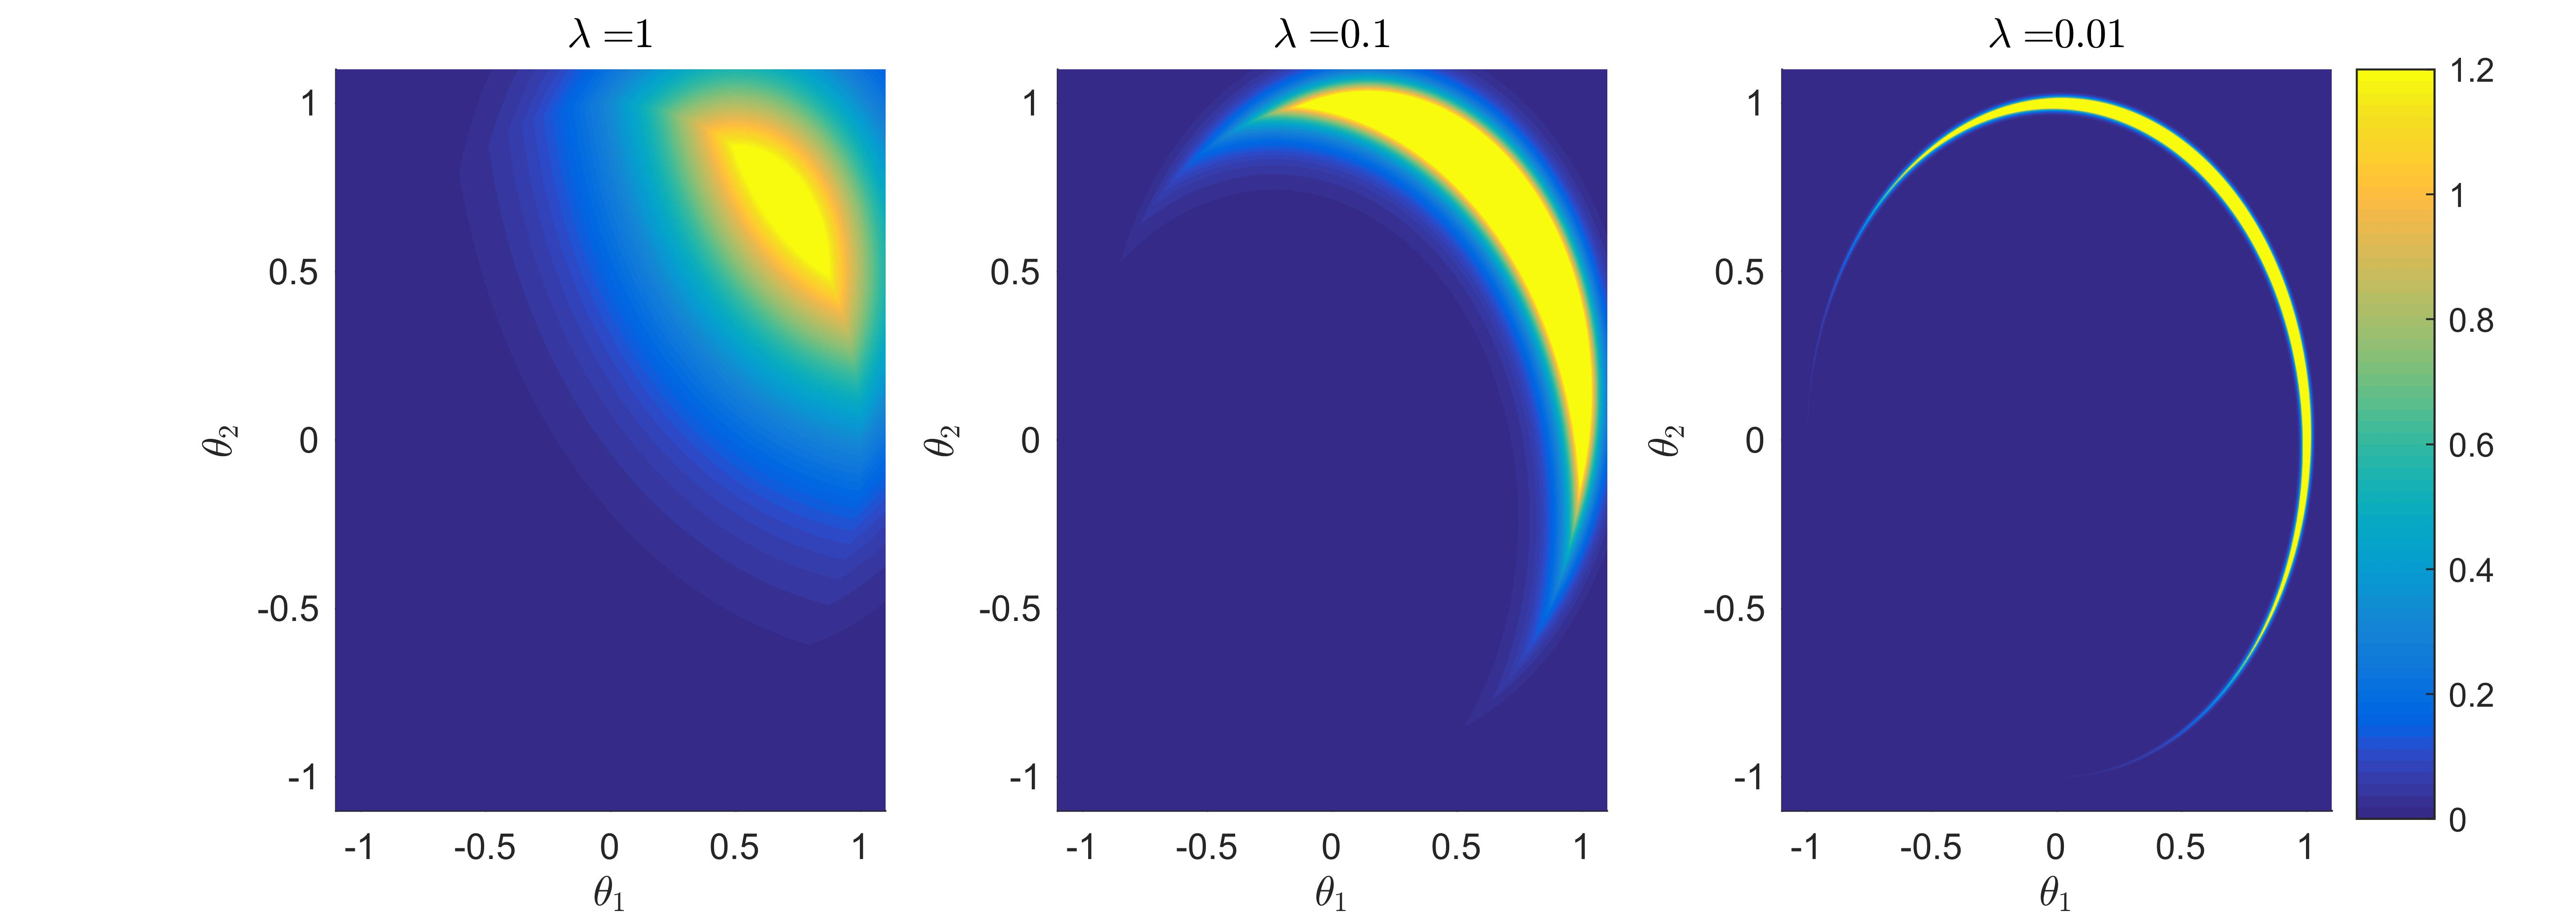
\includegraphics[width=1\textwidth]{Bivariate_Normal_Unit_Circle_Constraint}
		\caption{The relaxed distribution from Eq.
			\eqref{EQ:Relaxed_Density_Bivariate_Unit_Circle} for decreasing
			$\lambda$ is shown above when $\mu = (1/\sqrt{2},1/\sqrt{2})$ and $\sigma^2
				= 1/25.$  As $\lambda$ decreases, the relaxation is reduced
			and the circular constraint becomes clear.}
		\label{FIG:Bivariate_Normal_Unit_Circle_Constraint} \end{center}
\end{figure}

\section{Theory} 

In this section, we provide more theoretic justification for the proposed
method.

\subsection{Constrained
	Space with Positive Measure } \label{SEC:Positive_measure_theory}

	For constrained space with positive measure, we now focus on
	quantifying the difference between constrained and relaxed
	densities.  Both of these densities are absolutely continuous with respect to Lebesque
measure on $\mathcal{R}$.  Thus, the expectation of $g$ with respect to
constrained density is 

\begin{equation}
	\label{EQ:Expectation_Positive_Measure_Constraint}
	E[g(\theta)|\theta\in\mathcal{D}] = \int_\mathcal{D}
	g(\theta)\pi_\mathcal{D}(\theta)d\mu_\mathcal{R} =
	\frac{\int_\mathcal{D} g(\theta)\mathcal{L}(\theta; Y)
		\pi_\mathcal{R}(\theta)d\mu_\mathcal{R}(\theta)}{\int_\mathcal{D}
		\mathcal{L}(\theta; Y) \pi_\mathcal{R}(\theta)d\mu_\mathcal{R}(\theta)}.
\end{equation} 

Similarly, the expected value of $g$ with respect to the
relaxed density, 
\begin{equation} \label{EQ:Expectation_Positive_Measure_Relaxed}
	E_{\tilde{\pi}_\lambda}[g(\theta)] = \int_\mathcal{R}
	g(\theta)\tilde{\pi}_\lambda(\theta)d\mu_\mathcal{R} =
	\frac{\int_\mathcal{R} g(\theta)\mathcal{L}(\theta; Y)
		\pi_\mathcal{R}(\theta)
		\exp(-v_{\mc D}(\theta)/\lambda)d\mu_\mathcal{R}(\theta)}{\int_\mathcal{R}
		\mathcal{L}(\theta; Y)\exp(-v_{\mc D}(\theta)/\lambda)
		\pi_\mathcal{R}(\theta)d\mu_\mathcal{R}(\theta)}.\end{equation}

We can now consider the behavior of $E_{\tilde{\pi}_\lambda}[g]$ as
$\lambda \to 0^+.$

\begin{lemma} \label{THM:positive_measure_approximation_error} Suppose $g
		\in \mathbb{L}^1(\mathcal{R},
		\mathcal{L}(\theta;Y)\pi_\mathcal{R}d\mu_\mathcal{R})$.  Then,
	$$\bigg|E[g(\theta) |\theta\in\mathcal{D}] -
		E_{\tilde{\pi}_\lambda}[g(\theta)]   \bigg| \le
		\frac{\int_{\mathcal{R}\setminus \mathcal{D}}
		(C_\mathcal{R}E|g(\theta)|+|g(\theta)|) \mathcal{L}(\theta; Y)
		\pi_\mathcal{R}(\theta)\exp(-v_{\mc D}(\theta)/\lambda )
		d\mu_\mathcal{R}(\theta)}{\big[\int_\mathcal{D} \mathcal{L}(\theta; Y)
				\pi_\mathcal{R}(\theta)d\mu_\mathcal{R}(\theta)\big]^2 }$$ where
	$E|g(\theta)| \propto \int_\mathcal{R} |g(\theta)|
		\mathcal{L}(\theta;Y)\pi_\mathcal{R} d\mu_\mathcal{R}(\theta)$ is the
	expected value of $|g(\theta)|$ with respect to the unconstrained posterior
	density and $C_\mathcal{R} = \int_\mathcal{R}
		\mathcal{L}(\theta;Y)\pi_\mathcal{R}(\theta)d\mu_\mathcal{R}(\theta)$ is
	the normalizing constant of this unconstrained posterior density.
	Furthermore, if $v_{\mc D}(\theta)$ is zero for all $\theta\in\mathcal{D}$ and
	positive for $\theta\in(\mathcal{R}\setminus\mathcal{D})^o$, it follows
	from the dominated convergence theorem that $$\bigg|E[g(\theta)
		|\theta\in\mathcal{D}] - E_{\tilde{\pi}_\lambda}[g(\theta)]   \bigg|\to 0
		\text{ as } \lambda \to 0^+.$$ \end{lemma}

Thus, one can obtain sufficiently accurate estimates of
$E[g|\theta\in\mathcal{D}]$ by sampling from $\tilde{\pi}_\lambda$ when
$\lambda$ is sufficiently small.  From a practical standpoint, it is
desirable to understand the rate at which
$E_{\tilde{\pi}_\lambda}[g(\theta)] $ converges to
$E[g(\theta)\in\mathcal{D}]$. This question is addressed in the following
theorem.

\begin{theorem} \label{THM:Positive_measure_convergence_rate} Suppose $g
		\in  \mathbb{L}^2(\mathcal{R},
		\mathcal{L}(\theta;Y)\pi_\mathcal{R}d\mu_\mathcal{R})$,
	$v_{\mc D}(\theta)$ has the form of Eq. (\ref{EQ:Isotrophic_relaxation})
	with $k=2$, $\mathcal{D}$ has a piecewise smooth boundary, and that
	$\mathcal{L}(\theta;Y)\pi_\mathcal{R}(\theta)$ is continuous on a
	open neighborhood containing $\mathcal{D}$.  Then for $0<\lambda
		\ll 1,$ $$ \bigg|E[g(\theta) |\theta\in\mathcal{D}] -
		E_{\tilde{\pi}_\lambda}[g(\theta)]   \bigg| = O(\sqrt{\lambda}).  $$
\end{theorem} This theorem follows by applying the Cauchy-Schwartz
inequality to the term in the numerator of the bound given in Lemma
\ref{THM:positive_measure_approximation_error}.  One can attain a bound
depending on the surface area of $\mathcal{D}$ when it is bounded. The proofs of
Lemma \ref{THM:positive_measure_approximation_error} and Theorem
\ref{THM:Positive_measure_convergence_rate} are contained in Appendix
\ref{APP:Positive_Measure_Convergence_Proofs}.

These results have some important implications both analytically and
numerically.  First, in addition to point estimates,
$E[\theta \mid \theta\in\mathcal{D}]$, it is possible to approximate
probabilities $P(\theta \in \mathcal{F}|\theta \in \mathcal{D})$ and higher
moments, e.g. $E[\Pi_j \theta_j^{k_j} |\theta\in\mathcal{D}]$, so long as
these moments exist for the unconstrained posterior density.

Secondly, these bounds demonstrate that the error in using the relaxed
density to approximate $E[g(\theta)|\theta\in\mathcal{D}]$ is proportional
to $\sqrt{\lambda} [\int_\mathcal{D}\mathcal{L}(\theta; Y)
		\pi_\mathcal{R}(\theta)d\mu_\mathcal{R}(\theta)\big]^{-2}$ although this
rate may not be optimal.  In practice, $\lambda$ may need to be very small,
particularly in the case where $0<P(\theta\in\mathcal{D})\ll 1.$ Of course,
specific details of the scaling of $\bigg|E[g(\theta)
	|\theta\in\mathcal{D}] - E_{\tilde{\pi}_\lambda}[g(\theta)]   \bigg|$ will
depend upon the choice of $\mathcal{D}$ and $v_{\mc D}(\theta)$.

In general, one avenue for mitigating numerical difficulties which may
arise when $\lambda \ll 1$ is needed is to use 
\eqref{EQ:anistrophic_relaxation} to relax the density in directions where
accuracy is less important.  Fortunately, both Lemma
\ref{THM:positive_measure_approximation_error} and Theorem
\ref{THM:Positive_measure_convergence_rate} will still hold when the matrix $A$ is
positive definite since this corresponds to a  linear re-scaling of the
parameter space.


\subsection{Constrained Space with Zero Measure}
\label{SEC:Zero_measure_theory}

Before investigating the measure zero case, we review a few important concepts of
geometric measure theory which are used throughout this section.  First,
recall the definition of Hausdorff measure.  \begin{Hausdorff_def} Let
	$A\subset\mathcal{R}^r$. Fix $s \le r$. Then $$\mc H^{s}(A)=
		\underset{\delta\rightarrow 0}\lim \inf \bigg\{ \sum
		\left[{\text{diam}(S_i)}\right]^s: {A\subseteq \cup S_i,
		\text{diam}(S_i)\le \delta}, \text{diam}(S_i)=\sup_{x,y\in
			S}\|x-y\|\bigg\}$$.  \end{Hausdorff_def} We denote the normalized Hausdorff
measure as $\bar{\mc H}^{s}(A) =\frac{\Gamma(\frac{1}{2})^{s}}{2^s
		\Gamma(\frac{s}{2}+1)} \mc H^{s}(A)$. When $s=r$, Lebesgue and normalized
Hausdorff measures coincide  $\mu_{\mathbb{R}^m}(A)= \bar{\mc H}^{s}(A)$
\citep{evans2015measure}.  Additionally, for a subset $\mathcal{D}$, there
exists a unique, critical value $d$ such that
$$\bar{\mathcal{H}}^s(\mathcal{D}) = \begin{cases} 0, & s > d \\ \infty, &
		s < d.\end{cases}$$ The critical value, $d$, is referred to as the
Hausdorff dimension of $\mathcal{D}$. We note that, when $\mathcal{D}$ is a
compact, $d$-dimensional submanifold of $\mathbb{R}^m$, it will have
Hausdorff dimension $d$ and $\bar{\mathcal{H}}^d(\mathcal{D})$ is the
$d$-dimensional surface area of $A.$

We now state the co-area formula which is used to define a regular
conditional probability on the measure zero constrained space $\mathcal{D}$
and is pivotal in all of the proofs of the theorems.
\begin{theorem}{Co-area formula \citep{diaconis2013manifold,
			federer2014geometric}} Suppose $\nu:\mathbb{R}^r\to\mathbb{R}^s$
	with $ s<r$ is Lipschitz and that
	$g\in\mathbb{L}^1(\mathbb{R}^r,\mu_{\mathbb{R}^r}).$ Assume
	$J(\nu(\theta))>0$, then \begin{equation} \int_{\mathbb{R}^r}
		g(\theta)J\nu(\theta)d\mu_{\mathbb{R}^r}( \theta)=
		\int_{\mathbb{R}^s} \bigg( \int_{\nu^{-1}(y)}g(\theta)
		d\bar{\mathcal{H}}^{r-s}(\theta)\bigg)d\mu_{\mathbb{R}^s}(y),
	\end{equation} \end{theorem} The behavior of the pre-images
$\nu^{-1}(y)$ in the co-area formula are important for the
convergence results presented later in this section.  As such, we assume that $\mathcal{D}$ can be defined implicitly as the
solution set to a system of $s$ equations,  $\{\nu_j(\theta)=0\}_{j=1}^s$,
where \begin{itemize} \item[(a)] $\nu_j:\mathcal{R}\to\mathbb{R}$ is
	      Lipschitz continuous, \item[(b)] $v_j(\theta)=0$ only for
	      $\theta\in\mathcal{D}$, \item[(c)] for $k=1,\dots, s$, the preimage
	      $v_k^{(-1)}(x)$ is a co-dimension 1 sub-manifold of $\mathcal{R}$
	      for $\mu_\mathbb{R}$-a.e. $x$ in the range of $\nu_k$, \item[(d)]
	      $\nu_j^{(-1)}(0)$ and $\nu_k^{(-1)}(0)$ intersect transversally for
	      $1\le j<k\le s.$ \end{itemize} We refer to the functions
$\nu_1,\dots,\nu_s$ as constraint functions. In this case, if we
let $\nu:\mathcal{R}\to \mathbb{R}^s$ be the vector-valued function
$\nu(\theta) = [\nu_1(\theta),\dots,\nu_s(\theta)]^T$, then
$\mathcal{D} = \ker(v)$ is a co-dimension $s$ submanifold of
$\mathcal{R}$ for $\mu_{\mathbb{R}^s}$-a.e. $x$ the range of $v.$
Recall, the ambient space, $\mathcal{R}$, is $r-$dimensional.
Therefore, it follows that $\mathcal{D}$ is a $(r-s)-$dimensional
submanifold of $\mathcal{R}$, and it is natural to discuss the
$(r-s)$-dimensional surface area of $\mathcal{D}.$

Property (a), guarantees that $\nu$ is itself Lipschitz.  The remaining
properties (b)-(d) are constructed so that $\nu^{(-1)}(x)$ for
$x\in\mathbb{R}^s$ is also a submanifold which is close to
$\mathcal{D}=\nu^{(-1)}(0)$ when $x$ is near zero.  In particular, the
assumption of transversality ensures that $\nu^{(-1)}(x)$ with also be
$r-s$ dimensional for $x$ sufficiently close to 0.


The existence and uniqueness of the constraints must be addressed.  In the
case where $\mathcal{D}$ is specified by a collection of equality
constraints -- such as the probability simplex or the Stiefel manifold for
example--  it is not difficult to find a suitable set of constraint
functions. Table \ref{TABLE:Equality_constraints_examples} contains a
number of examples of common constrained spaces and appropriate choices of
constraint functions.  \renewcommand{\arraystretch}{1.5} \begin{table}[h!]
	\begin{center} \begin{tabular}{| c | m{4 cm} | c | c | m{6cm} |}
			\hline $\mathcal{R}$                           & $\mathcal{D}$                                  & $\dim(R)$ &
			$\dim(D)$                                      & Constraint functions                                                        \\ \hline $[0,1]^r$ &
			Probability simplex, $\Delta^{r-1}$                 & $r$                                            & $r-1$     & $v(\theta)
				= \sum(\theta) -1$                                                                                                           \\ \hline $\mathbb{R}^r$ & Line,
			span$\{\vec{u}\}$ \newline $\vec{u}\ne\vec{0}$ & $r$                                            & $1$
			                                               &
			$\nu_j(\vec{\theta}) = \vec{\theta}\,^T\vec{b}_j$ \newline
			$\{\vec{b}_1,\dots,\vec{b}_{r-1}\}$ a basis for
			span$\{\vec{u}\}^\perp$                                                                                                      \\ \hline $[-1,1]^r$ & Unit
			sphere, $\mathbb{S}^{r-1}$                     & $r$                                            & $r-1$     & $v(\theta) =
				(\|\theta\|^2 -1)$                                                                                                    \\ \hline $[-1,1]^{n\times
			k}$                                            & Stiefel manifold, $V_k(\mathbb{R}^n)$ \newline
			$\theta = [\vec{\theta}_1 | \dots | \vec{\theta}_k], \,
			\vec{\theta}_j \in \mathbb{R}^n$               & $nk$                                           & $nk -
			\frac{1}{2}k(k+1)$                             & $v_{i,j}(\theta) = (
				\vec{\theta}_i'\vec{\theta}_j- \delta_{i,j})$ \newline
			$1\le i \le j \le k$ and $\delta_{i,j} = \mathbbm{1}_{i=j}$
			\\ \hline\end{tabular} \end{center} \caption{Table of
		constraints for some commonly used constrained spaces.}
	\label{TABLE:Equality_constraints_examples} \end{table}

% In the more difficult situation where equality constraints are not given,
% finding $\{\nu_j\}_{j=1}^s$ may be very challenging. For the moment, we
% will assume that one can construct sufficiently accurate numerical
% approximations perhaps through cubic-splines or Fourier series, so that we
% may ignore the issue of existence.

With regards to uniqueness, we note that the constraints cannot be unique
in any case.  For example, rescaling in each $v_j(\theta)$ will also satisfy (a)-(d). Naturally, an optimal choice will depend largely on the properties of the
constrained distribution that one wishes to estimate making the choice of
$\{\nu_j\}_{j=1}^s$ context dependent.

Under the given construction of the constrained space, we can now specify
the regular conditional probability of $\theta$, given $\theta \in
	\mathcal{D}.$ 

	\begin{theorem}\citep{diaconis2013manifold}
	\label{THM:RCP_construction} Assume that $J(v(\theta)) > 0$ and
	that for each $z\in\mathbb{R}^s$ there is a finite non-negative
	 $p_z$ such that,  $$m^{p_z}(z) = \int_{v^{-1}(z)}
		\frac{\mathcal{L}(\theta; Y) \pi_\mathcal{R}(\theta)}
			{J(v(\theta))} d\bar{\mathcal{H}}^{p}(\theta)
		\in (0,\infty).$$ 

		Then, for any Borel subset $E$, of
	$\mathcal{R}$, it follows that $$P(E \mid v(\theta) = z) = \begin{cases}
			\frac{1}{m^{p_z}(z)} \int_E \frac{\mathcal{L}(\theta; Y)
				\pi_\mathcal{R}(\theta)
				\mathbbm{1}_{v(\theta)=z}}{J(v(\theta))} d\bar{\mathcal{H}}^{p}(\theta)
			 & m^p(z)\in (0,\infty) \\ \delta (E) & m^p(z) \in \{0,\infty\}
		\end{cases}$$ 
		is a valid regular conditional probability for
	$\theta\in\mathcal{D}.$ Here, $\delta (E)=1$ if $0\in E$ and $0$ otherwise.
\end{theorem}

By construction, $\{\theta:v(\theta)=z\}$ is a $(r-s)$ dimensional
submanifold of $\mathcal{R}$ for $\mu_{\mathbb{R}^s}$-a.e. $z$ in $\mc X$, the range
of $v$. As such, it follows that one should take $p_z=r-s$. It is possible that
$m^p(z)\in\{0,\infty\}$ for some $z\not\in \mc X$; however, they are excluded during our construction. See Diaconis et al. (2013)
for additional discussion of this issue. Most importantly, $0\in \mc X$, therefore, Theorem~\ref{THM:RCP_construction} allows us to define

\begin{equation} \label{EQ:Constrained_rcp}
	\pi_\mathcal{D}(\theta|\theta\in\mathcal{D},Y) = \frac{1}{m^{r-s}({0})}
	\frac{\mathcal{L}(\theta; Y) \pi_\mathcal{R}(\theta)
	\mathbbm{1}_{v(\theta)={0}}}{J(v(\theta))} \end{equation} as the
constrained posterior density.

 As a result, we
can define the conditional  expectation of $g(\theta)$ given $\theta \in
	\mathcal{D}$ as $$E[g(\theta) | \theta\in\mathcal{D}] = E[g(\theta) |
			\nu(\theta) =0\,] = \int_\mathcal{R} g(\theta) \pi_\mathcal{D}(\theta)
	d\bar{\mathcal{H}}^{r-s}(\theta).$$

The expected value of
$g(\theta)$ with respect to the relaxed density, denote
$E_{\tilde{\Pi}}[g(\theta)] $, is

$$		E_{\tilde{\Pi}}[g(\theta)] = \frac{1}{m_\lambda}
		\int_\mathcal{R} g(\theta) \pi_\mathcal{R}(\theta)
		\mathcal{L}(Y;\theta)\exp\bigg(-\frac{1}{\lambda}\|\nu (\theta)\|_1\bigg)
		d\mu_\mathcal{R}(\theta) $$
		with $m_\lambda =
	\int_\mathcal{R}  \pi_\mathcal{R}(\theta)
	\mathcal{L}(Y;\theta)\exp\bigg(-{\lambda^{-1}}\|\nu (\theta)\|_1\bigg)
	d\mu_\mathcal{R}(\theta).$
The primary results of the section are the following statements regarding
the use of $E_{\tilde{\Pi}}[g]$ to estimate $E[g|\theta\in\mathcal{D}]$.

\begin{theorem} \label{THM:Relaxed_Expectation_Convergence_Measure_Zero}
	Let $m:\mathbb{R}^s\to \mathbb{R}$ and $G:\mathbb{R}^s\to
		\mathbb{R}$ be defined as follows \begin{align*} m(x) & =
		\int_{\nu^{-1}(x)} \frac{\pi_\mathcal{R}(\theta)
			\mathcal{L}(y;\theta)}{J(\nu(\theta))}
		d\mathcal{R}^{r-s}(\theta) \\ G(x) &= \int_{\nu^{-1}(x)}
		g(\theta)\frac{\pi_\mathcal{R}(\theta)
			\mathcal{L}(y;\theta)}{J(\nu(\theta))} d\mathcal{R}^{r-s}(\theta).
	\end{align*} Suppose that both $m$ and $G$ are continuous on an open
	interval containing the origin and that \\
	$g\in\mathbb{L}^1(\mathcal{R},\pi_R\mathcal{L}(y;\theta)d\mu_\mathcal{R})$.
	Then, $$\bigg|E_{\tilde{\Pi}}[g] - E[g|\theta \in \mathcal{D}]\bigg| \to 0
		\text{ as } \lambda\to 0^+.$$ \end{theorem}

\begin{corollary} In addition to the assumptions of Theorem
	\ref{THM:Relaxed_Expectation_Convergence_Measure_Zero}, suppose
	that both $m$ and $G$ are differentiable at $0$. Then
	$$\bigg|E_{\tilde{\Pi}}[g] - E[g|\theta \in \mathcal{D}] \bigg| =
		O\bigg(\frac{\lambda}{|\log \lambda|^s}\bigg)$$ as $\lambda \to
		0^+.$ \end{corollary}

Like the results from Section 3.1, the convergence rates are sub-linear.
However, unlike the positive measure case, the convergence rates are
dimension dependent.


\section{Posterior Computation}

Compared to constrained density in  space $\mc D$, relaxed density is supported in $\mc R$ and can be directly 
sampled via off--the--shelf tools such as slice
sampling, adaptive Metropolis-Hastings and Hamiltonian Monte Carlo (HMC).
In this section, we focus on HMC for its easiness to use and good
performance in block updating of parameters.

\subsection{Hamiltonian Monte Carlo under Constraint Relaxation}

We provide a brief overview of HMC for continuous $\theta^*$ under
constraint relaxation. Discrete extension is possible via recent work of
\cite{nishimura2017discontinuous}.

In order to sample $\theta$, HMC introduces an auxillary momentum variable $p
	\sim \No(0, \mass)$. The covariance matrix $\mass$ is referred to as a
\textit{mass matrix} and is typically chosen to be the identity or adapted
to approximate the inverse covariance of $\theta$. HMC then sample from the
joint target density $\pi(\theta, p) = \pi(\theta) \pi(p) \propto \exp (- H(\theta, p))$
where, in the case of the posterior under relaxation,


\begin{equation} \begin{aligned}
		H(\theta, p) & = U(\theta)+K(p), \\ \text{where } &
		U(\theta) = -\log\pi(\theta),    \\ & K(p) = \frac{p'\mass^{-1} p}{2}.
	\end{aligned}
\end{equation}
with $\pi(\theta)$ is the unnormalized density in \eqref{EQ:relaxedDensityPosMeasure} or \eqref{EQ:relaxedDensityZeroMeasure}.

From the current state $(\theta^{(0)},p^{(0)})$, HMC generates a proposal for
Metropolis-Hastings algorithm by simulating Hamiltonian dynamics, which is
defined by a differential equation:

\begin{equation} \begin{aligned} \label{hamiltonian} \frac{\partial \theta
		^{(t)}}{\partial t} & =\frac{\partial H(\theta, p)}{\partial p} =
		\mass^{-1}p,                                                 \\ \frac{\partial p^{(t)}}{\partial t}&
		=-\frac{\partial H(\theta, p)}{\partial \theta} = -\frac{\partial
			U(\theta)}{\partial \theta}.\end{aligned} \end{equation}

The exact solution to \eqref{hamiltonian} is typically intractable but a
valid Metropolis proposal can be generated by numerically approximating
\eqref{hamiltonian} with a reversible and volume-preserving  integrator
\citep{neal2011mcmc}. The standard choice is the \textit{leapfrog}
integrator which approximates the evolution $(\theta^{(t)},p^{(t)}) \to (\theta^{(t +
			\dt)},p^{(t + \dt)})$ through the following update equations:

\begin{equation} \begin{aligned} \label{leap-frog} 
p \leftarrow p -
		\frac{\dt}{2} \frac{\partial U}{\partial  \theta },\quad \theta \leftarrow  \theta
		+ \dt \mass^{-1}p,\quad p \leftarrow p -  \frac{\dt}{2}
		\frac{\partial U}{\partial  \theta }\end{aligned} \end{equation} Taking
$L$ leapfrog steps from the current state $(\theta^{(0)},p^{(0)})$
generates a proposal $(\theta^{*},p^{*}) \approx (\theta^{(L \dt)},p^{(L
	\dt)})$, which is accepted with the probability $$1\wedge \exp
	\left( - H(\theta^{*},p^{*}) + H(\theta^{(0)},p^{(0)}))\right)$$

We refer to this algorithm as CORE-HMC.

\subsection{Computing Efficiency in CORE-HMC}

Since CORE expands the support from $\mc D$ to $\mc R$, it is useful to
study the effect of space expansion on the computing efficiency of HMC. In this
subsection, we provide some  quantification of the effects.


In understanding the computational efficiency of HMC, it is useful to
consider the number of leapfrog steps to be a function of $\dt$ and set $L
	= \lfloor \tau / \dt \rfloor$ for a fixed integration time $\tau > 0$. In
this case, the mixing rate of HMC is completely determined by $\tau$ in the
limit $\dt \to 0$ \citep{betancourt17}. In practice, while a smaller
stepsize $\dt$ leads to a more accurate numerical approximation of
Hamiltonian dynamics and hence a higher acceptance rate, it takes a larger
number of leapfrog steps and gradient evaluations to achieve good mixing.
For an optimal computational efficiency of HMC, therefore, the stepsize
$\dt$ should be chosen only as small as needed to achieve a reasonable
acceptance rate \citep{beskos13, betancourt14}. A critical factor in
determining a reasonable stepsize is the \textit{stability limit} of the
leapfrog integrator \citep{neal2011mcmc}. When $\dt$ exceeds this limit,
the approximation becomes unstable and the acceptance rate drops
dramatically. Below the stability limit, the acceptance rate $a(\dt)$ of
HMC increases to 1 quite rapidly as $\dt \to 0$ and in fact satisfies
$a(\dt) = 1 - \mc O(\dt^4)$ \citep{beskos13}.

For simplicity, the following discussions assume the mass matrix $\mass$ is
taken to be the identity, and $\mc D= \cap_{j=1}^s\{\theta :v_j(\theta)=0 \}$.
We denote $\mc D_j= \{\theta :v_j(\theta)=0 \}$ and use directional relaxation
$\exp(-\sum_j{\|v_j(\theta^*)\|}{\lambda_j^{-1}})$. There are generally two factors limiting the efficiency of HMC:
(i) the width of support in constrained space; (ii) the largest eigenvalue of the Hessian matrix.
For the former, using $\mc Q$ to denote a support, the width of support is related to the shortest
distance to the boundary $\eta (\theta; {\mc Q})= \inf_{\theta'\not\in \mc
		Q}\|\theta'-\theta\|$. If $\eta (\theta; {\mc Q}) \approx 0$ for all $\theta\in \mc Q$,
		 the proposal would likely be rejected using a large leap-frog step size. In such case, 
		 it is useful to utilize CORE to expand support and  
increase $\eta (\theta; {\mc Q})$ for better computing efficiency. For the eigenvalue,
let $\hess_U(\theta)$ denote the hessian matrix of
$U(\theta) = - \log \pi(\theta)$. 
The linear stability analysis and
empirical evidences suggest that, for stable approximation of Hamiltonian
dynamics by the leapfrog integrator in $\bb R^p$, the condition $\dt <
	2\xi_1(\theta)^{-1/2}$ must hold on most regions of the parameter space
\citep{hairer06}, with $\xi_1(\theta)$ the largest
eigenvalue of $\hess_U(\theta)$. The hessian is

\begin{equation} \label{eq:hessian_extrinsic}
 \hess_U(\theta) = -\hess_{\log
		(\mathcal L(\theta;y) \pi_{\mc R}(\theta))
	}(\theta)+\sum_j \lambda_j^{-1} \hess {\|v_j(\theta)\|}
	\mathbbm{1}_{\theta\not\in \mc D_j}. \end{equation}
Note the second term is zero unless $\theta$ is outside of $\mc D_k$. As $\lambda^{-1}_j$ in the
second term often dominates the eigenvalue in the first term, hence the effective eigenvalue often is
proportional to $ \underset{j: \theta \not\in \mc D_j}{\min}\lambda_j^{1/2}$.

Lastly, one often may want to use CORE for obtaining approximate estimate under constrained model.
For this purpose, we now provide a practical guidance on choosing $\lambda_j$.  For $\mc
D_j$'s with very small distance to support boundary $\eta(\theta;\mc D_j)\approx 0$, one should use moderate $\lambda_j$
to increase support width;  for $\mc D_j$'s
without this issue, one should use very small $\lambda_j\approx 0$ to keep $\theta\in\mc D_j$, so that it has almost no influence on the hessian eigenvalue. 
To prevent high rejection of HMC near the boundary of $\mc D_j$, we suggest random step size $\epsilon$ at each iteration to
reduce the error, which is typically recommended in HMC \citep{neal2011mcmc}. When space expansion is exploited, a trade-off between approximation accuracy
and computational efficiency is involved. Empirically, we found reducing
$\lambda_{j}$ $10$ to times smaller requires approximately $3$ times more
computing time.


\section{Simulated Examples}

The simple computation of CORE frees up the modeling flexibility. We now illustrate more utility of the method via simulated examples.

\textbf{Example: Sphere $t$ Distribution}

We now derive a new distribution on a $(p-1)$-sphere $\mc
D=\{\theta\in
\bb R^p:\|\theta\|_2 =1\}$. Recall that von
Mises--Fisher distribution \citep{khatri1977mises} is the result of constraining a multivariate Gaussian $\theta \sim \No(F,I\sigma^2)$ to $\mc D$

$$
\pi_{\mc D}(\theta) \propto
\exp(-\frac{\|F-\theta\|^2}{2\sigma^2})
\mathbbm{1}_{\theta'\theta=1} \\
 \propto
\exp(\frac{F'}{\sigma^2}\theta)
\mathbbm{1}_{\theta'\theta=1}.
$$
 Although the final form
appears more
like an exponential, the behavior of von
Mises--Fisher
on sphere can be largely explained by its unconstrained parent Gaussian.
In the Gaussian $\pi_{\mc
R}(\theta)$, $\theta$ is symmetrically distributed around $F$, with density
decaying exponentially as $\| \theta-F\|^2$ increases with rate 
$({2\sigma^2})^{-1}$; as the constrained
density $\pi_{\mc D}(\theta)$ is proportional $\pi_{\mc R}(\theta)$, it concentrates
similarly. 

This naturally suggests we could use another distribution to induce different behavior on the sphere; then one could use CORE to generate approximate sample. We start from a
multivariate $t$-distribution $\pi_{\mc
R}(\theta)$, $t_m(F,I\sigma^2)$ with $m$ degrees of freedom,
mean $F\in \mc D$ and variance $I\sigma^2$, using \eqref{EQ:Constrained_rcp} to generate a density 
\be
\pi_{\mc
D}(\theta)
\propto &
(1+\frac{\|F-\theta\|^2}{m\sigma^2})^{-\frac{(m+p)}{2}}\mathbbm{1}_{\theta'\theta=1}\\
\propto &
(1-\frac{F'\theta}{1+m\sigma^2/2})^{-\frac{(m+p)}{2}}\mathbbm{1}_{\theta'\theta=1}
\ee
As in the $t$-distribution, the density decays polynomially as $\|F-\theta\|^2$ increases, as opposed to the exponential decay in Gaussian. We refer to this new distribution as sphere $t$-distribution.

CORE allows us to easily obtain approximate sample via relaxation function $\exp(- \lambda^{-1}\|\theta'\theta-1\|)$. Figure~\ref{sphere_examples} shows that the sphere t-distribution with $m=3$ exhibits much less concentration than von Mises--Fisher on the sphere,. This can be useful for robust modeling when there could be `outlier' on the sphere.
\begin{figure}[H]
\begin{subfigure}[b]{0.45\textwidth}
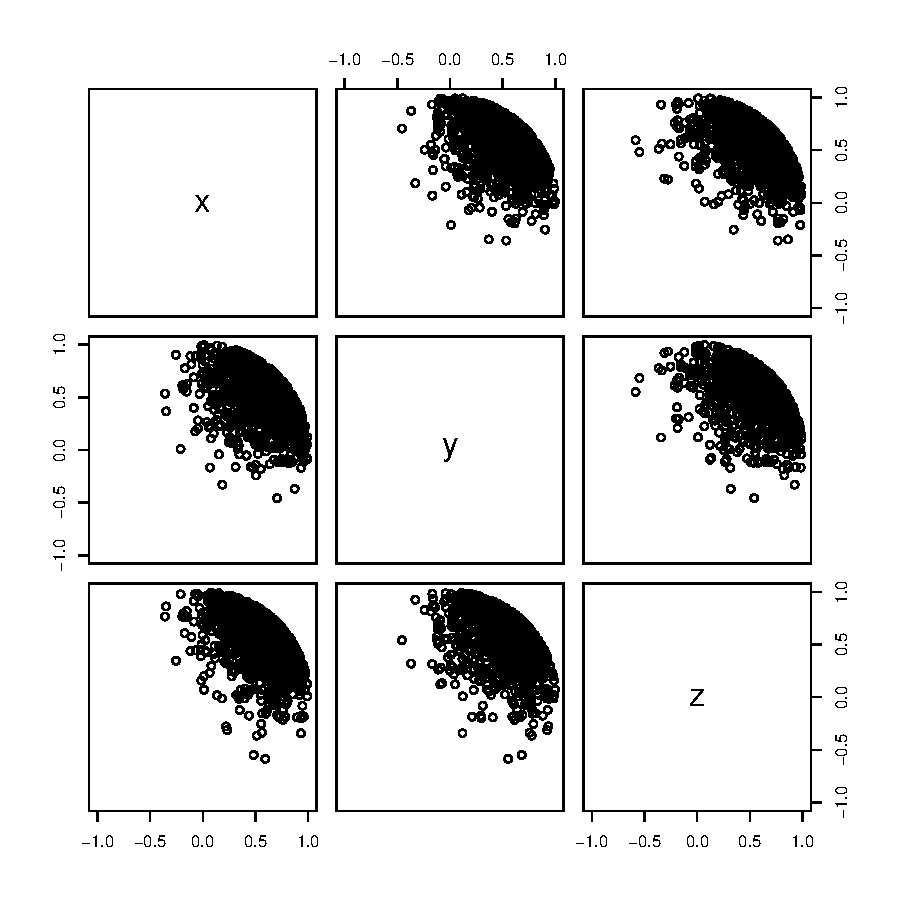
\includegraphics[width=1\textwidth]{sphere_vmf.pdf}
\caption{von Mises--Fisher distribution.}
\end{subfigure}
\begin{subfigure}[b]{0.45\textwidth}
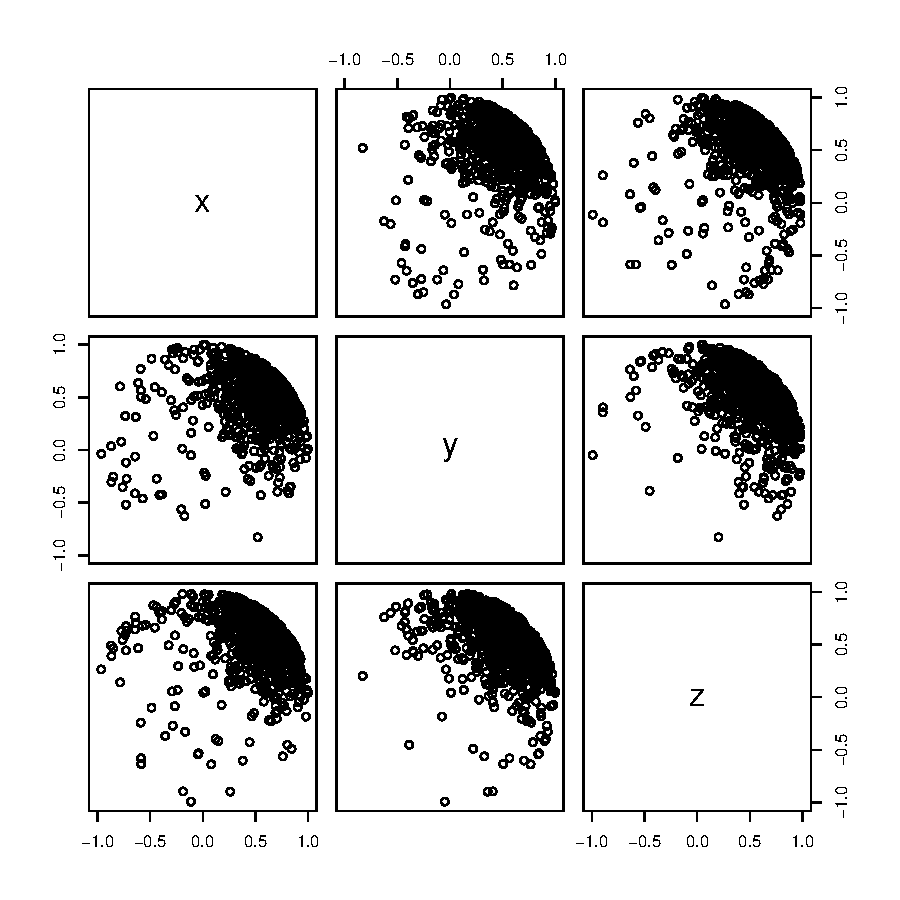
\includegraphics[width=1\textwidth]{sphere_t}
\caption{Sphere $t$-distribution with $m=3$.}
\end{subfigure}
\caption{Sectional view of random samples from constrained distributions on a unit sphere inside $\bb R^3$. The distributions are derived through conditioning on $\theta'\theta=1$ based on unconstrained densities of (a) $\No( F, \diag\{0.1\})$, (b) $t_3(F,\diag\{0.1\} )$, where $F=[1/\sqrt{3},1/\sqrt{3},1/\sqrt{3}]'$. The samples are generated via CORE-HMC with $\lambda=10^{-3}$.
}
\label{sphere_examples}
\end{figure}

\textbf{Example: Ordered Dirichlet Distribution}

We derive an ordered Dirichlet distribution. We build it upon the canonical Dirichlet distribution $\mbox{Dir}(\alpha)$ with $
\pi_{\mc D}(\theta) \propto \prod_{j=1}^J \theta_j^{\alpha-1} \1_{\sum_{j=1}^J \theta_j=1}$ and further impose order constraint, $1> \theta_1 \ge \ldots \ge \theta_J > 0$, yielding


 \begin{equation}
\begin{aligned}
\label{ordered_dp_prior}
\pi_{\mc D}(\theta) \propto \prod_{j=1}^J \theta_j^{\alpha-1} \cdot \1_{\sum_{j=1}^J \theta_j=1} \cdot  \prod_{j=1}^{J-1}\1_{\theta_j \ge \theta_{j+1}}.
\end{aligned}
\end{equation}

As commonly used in mixture model, canonical Dirichlet prior has its index $j$ exchangeable. Since its permutation does not change the likelihood, label-switching problem often occurs (reviewed in \cite{jasra2005markov}). Naturally, order constraint in $\theta$ can alleviate this problem, especially in preventing the switch between large $\theta_j$ and small $\theta_{j'}$.

To illustrate, we consider a hierarchical normal distribution with a common variance but the mean from a mixture, for data $y_i\in \bb R^2$ indexed by $i=1,\ldots,n$:

\begin{equation*}
\begin{aligned}
y_i &\stackrel{indep}{\sim} \No(\mu_i,\Sigma),\qquad
\mu_i &\stackrel{iid}{\sim} G,\qquad
G(.) & = \sum_{j=1}^{J} \theta_j \delta_{\mu_j}(.),
\end{aligned}
\end{equation*}

We generate $n=100$ samples from $3$ components with $\{\theta_1,\theta_2,\theta_3\}=\{0.6,0.3,0.1\}$, $\{\mu_1,\mu_2,\mu_3\} = \{[1,5], [3,3], [3,5]\}$ and $\Sigma = I_2$. We assign weakly informative priors $\No(0,10 I_2)$ for each $\mu_j$ and inverse--Gamma prior for the diagonal element in $\Sigma=\diag(\sigma_1^2,\sigma_2^2)$ with $\sigma^2_1, \sigma^2_2\sim \mbox{IG}(2,1)$.  Figure~\ref{dirichlet}(a) shows the contour of posterior density of $\mu$. The small component sample size leads to large overlap among the posterior. 


\begin{figure}[H]
\begin{center}
   \begin{subfigure}[b]{0.6\textwidth}
    \centering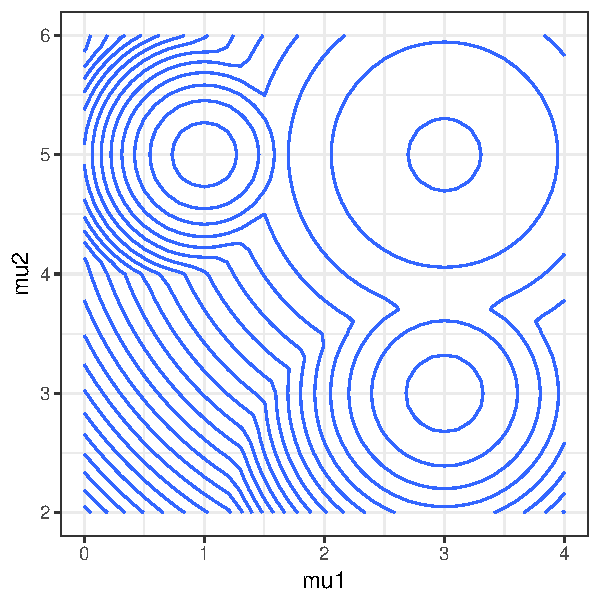
\includegraphics[width=0.5\textwidth]{fmm_mu_contour.pdf}
    \caption{\small Posterior density of the component means $\{\mu_j\}_{j=1}^3$.}
    \end{subfigure}
    \end{center}
    \centering
   \begin{subfigure}[b]{0.32\textwidth}
    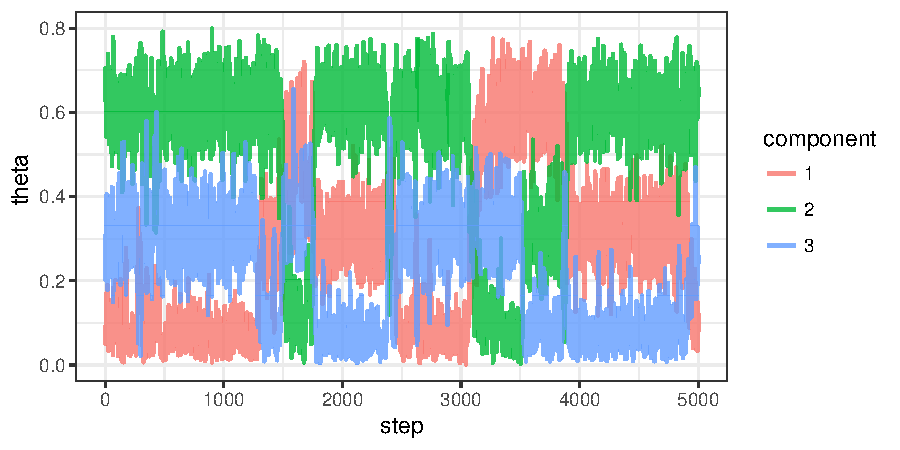
\includegraphics[width=1\textwidth]{fmm_w_gibbs.pdf}
    \caption{\small  Gibbs sampling of unordered Dirichlet}
    \end{subfigure}
       \begin{subfigure}[b]{0.32\textwidth}
  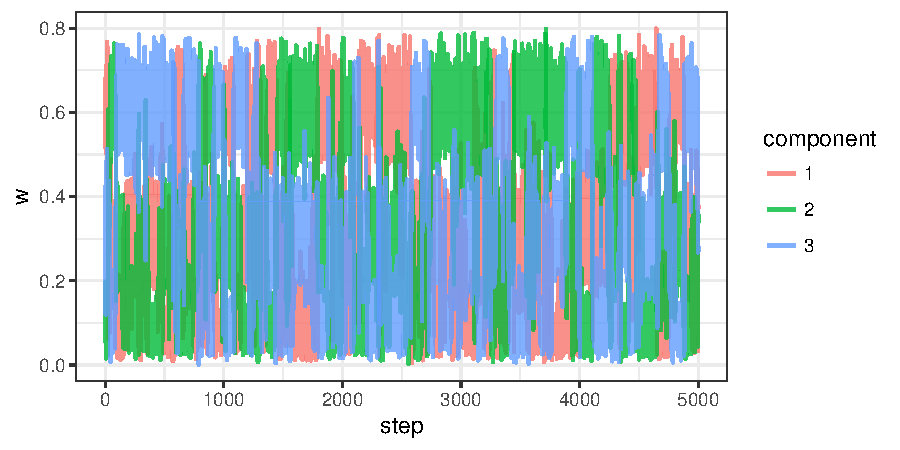
\includegraphics[width=1\textwidth]{fmm_w_hmc_unordered.pdf}
    \caption{\small  HMC sampling of unordered Dirichlet}
      \end{subfigure}
       \begin{subfigure}[b]{0.32\textwidth}
 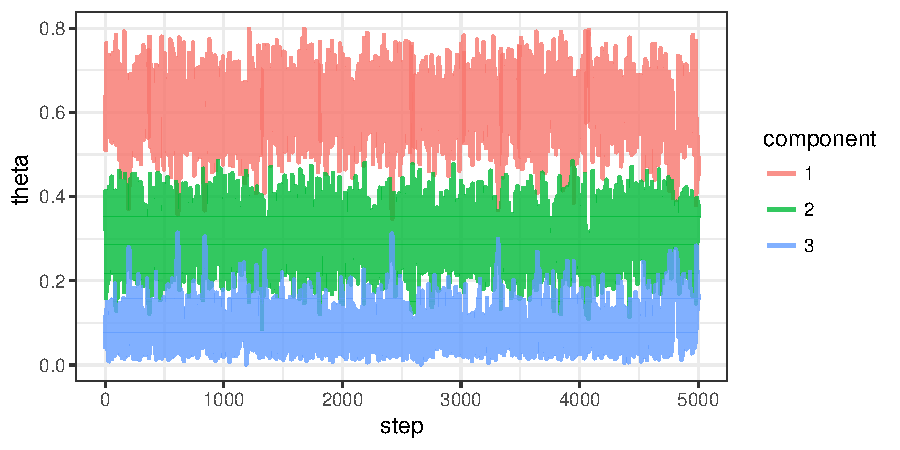
\includegraphics[width=1\textwidth]{fmm_w_hmc.pdf}
     \caption{\small  HMC sampling of ordered Dirichlet}
     \end{subfigure}
\caption{Contour of the posterior density of component means and traceplot of the posterior sample for the component weights $w$, in a 3-component normal mixture model. Panel (a) shows that there is significant overlap among component means $\{\mu_j\}_{j=1}^3$. Without ordering in $\theta$, its traceplot shows label-switching issue in both Gibbs (b) and HMC  (c) sampling of Dirichlet distribution. The ordered Dirichlet distribution has significantly less label-switching issue (d), where we utilize CORE to obtain approximate posterior sample.}
\label{dirichlet}
\end{figure}


The ordering disrupts the traditional Gibbs sampling \citep{ishwaran2001gibbs}, however, one could still obtain approximate posterior using CORE. We use $
\exp ( -  {\lambda_1}^{-1} \| \sum_{j=1}^J  \theta_{j} - 1) \|)
\prod_{j=1}^{J-1} \exp [ -  {\lambda_2}^{-1}  \max( \theta_{j+1} - \theta_j,0)]  $ to relax the constraints. We use $\lambda_1 = 10^{-3}$ on simplex constraint to allow efficient sampling and $\lambda_2 = 10^{-6}$ to induce almost no relaxation on the ordering.

We compare the traceplots of ordered Dirichlet and unordered Dirichlet. Without the order constraint, significant label-switching occur in both Gibbs and HMC (traceplots in Figure~\ref{dirichlet}(b,c)), whereas ordered Dirchlet has almost no label-switching( Figure~\ref{dirichlet}(d)).

\section{Application: Finding Sparse Basis in a Population of Networks}

We now consider a real data application in brain network analysis.  The
brain connectivity structures are obtained in the data set KKI-42 (Landman
et al. 2011), which consists of $n=21$ healthy subjects without any
history of neurological disease. We take the first scan out of the
scan-rescan data as the input. Each observation is a $V\times V$ symmetric
network, recorded as an adjacency matrix $A_i$ for $i=1,\ldots,n$. The
regions are constructed via the Desikan et al. (2006) atlas, for a total
of V = 68 nodes.  For the $i$th matrix $A_i$, $A_{i,k,l} \in \{0,1\}$ is
the element on the $k$th row and $l$th column of $A_i$, with
$A_{(i,k,l)}=1$ indicating there is an connection between $k$th and $l$th
region, $A_{(i,k,l)}=0$ if there is no connection. The matrix is symmetric
due to the undirectedness of the network, but the diagonal records
$A_{(i,k,k)}$ for all $i$ and $k$ are missing due to the lack of meaning
for self-connectivity.


One scientific interest in neuroscience is to quantify the variation of
brain networks and identify the  regions (nodes) that contribute to it.
Extending factor analysis to multiple matrices, one appealing approach is
to have the networks share a common factor matrix but let the  loadings
vary across subjects. This can be considered as a simplified equivalent of
three-way tensor factorization \citep{kolda2009tensor}. Then to selectively
identify the important nodes, one natural way is to apply shrinkage on the
elements of factor matrix.


Geometrically, the factor matrix, denoted by $\{U_1,\ldots,U_d\},$ reside
on a Stiefel manifold $\mc V(n,d)=\{U: U'U=I_d\}$, where
$U=[U_1,\ldots,U_d]$ is the $n\times d$ matrix. Using $r$ to index
$1,\ldots,d$, each frame $U_r$ represents a $(n-1)$-hypersphere. Applying
shrinkage forces some of its sub-coordinates to be close to $0$, which is
reducing each $U_r$ onto a lower-dimensional hypersphere.  Although
previous work was done using sparse PCA \citep{zou2006sparse} for
continuous outcome,  little work has been done in a probabilistic model for
binary matrices.

To apply shrinkage in the constrained space, we adopt the induced prior  as
common in Bayesian  literature (reviewed by \cite{polson2012local}), which
usually takes the form hierarchical structure $\theta_i\mid \kappa_i
	,\sigma\sim \No(0,\kappa_i \sigma), \quad \kappa_i\sim G_1, \quad \sigma
	\sim G_2$ with $\kappa_i$, $\sigma$ as the local and global scale
parameters.  However, when constraining $\theta_i$, one caveat would be
only adapting the conditional density $\No(\theta_i;\kappa_i \sigma)$,
which  yields intractable normalizing constant involving $\kappa_i \sigma$
in the conditional. This difficulty can be avoided by reparameterizing\
$\theta_i=\eta_i\kappa_i\sigma$ with $\eta_i\sim\No(0,1)$, and adapting the
	{\it joint} density of $\{\eta_i,\kappa_i,\sigma\}$ on constrained space
instead. The joint density will not have intractable constant as long as
the hyper-parameters in $G_1$ and $G_2$ are fixed.

We now take the Dirichlet-Laplace prior \citep{bhattacharya2015dirichlet}
as unconstrained distribution $\pi_{\mc R}$ and adapt it onto Stiefel
manifold via \eqref{constrainedDensity}.  \begin{equation*} \begin{aligned}
		 & A_{(i,k,l)} \sim \text{Bern}( \frac{1}{1+ \exp(-\psi_{(i,k,l)}-
			z_{(k,l)})})                                                       \\ & \psi_{(i,k,l)} = \sum_{r=1}^{d}  v_{(i,r)} u_{(k,r)}
		u_{(l,r)}                                                          \\ & U'U=I_{d} \text{ with } U=\{u_{(k,r)}\}_{k=1,\ldots,n;
		r=1,\ldots,d}                                                      \\ & u_{(k,r)}= \eta_{(k,r)}\kappa_{(k,r)}\sigma_{u} \\ &
		\eta_{(k,r)}\sim \text{Lap}(0,1), \quad \{\kappa_{(1,r)}\ldots
		\kappa_{(V,r)}\} \sim \text{Dir}(\alpha), \quad \sigma^2_{u}\sim
		\text{IG}(2,1)                                                     \\   & z_{(k,l)} \sim \No(0,\sigma^2_z), \quad  \sigma^2_z
		\sim \text{IG}(2,1)                                                \\ & v_{(i,r)} \sim \No(0,\sigma^2_{v,(r)}), \quad
		\sigma^2_{v,(r)} \sim \text{IG}(2,1)\end{aligned} \end{equation*} for
$k>l$, $k=2,\ldots, V$, $i=1,\ldots,n$;  $\text{Lap}(0,1)$ denotes the
Laplace distribution centered at $0$ with scale $1$;
$Z=\{z_{(k,l)}\}_{k=1,\ldots,V;l=1,\ldots,V}$ is a symmetric unstructured
matrix that serves as the latent mean; $\{ v_{(i,r)}\}_{r=1,\ldots,d}$ is
the loading for the $i$th network, with each $v_{(i,r)}>0$; for all other
scale parameters $\sigma^2_.$, we choose weakly informative prior inverse
Gamma $\text{IG}(2,1)$, as appropriate for the scale under the logistic
link. To induce sparsity in each Dirichlet, we use $\alpha=0.1$ as
suggested by \cite{bhattacharya2015dirichlet}.


There are two types of constraints in the model,  $U'U=I_d$ and
$\sum_{k=1}^V \kappa_{(k,r)}=1$ for $r=1,\ldots,d$. Taking $v_1(U)=
	U'U-I_d$ and $v_2(\kappa_{(k,r)})=\sum_{k=1}^V \kappa_{(k,r)}-1$ for each
$r$, the Jacobian is  constant in \eqref{constrainedDensity}. For posterior
computation, we use DA-CORE as described above.  Using latent variable
$w_U$ $d$-by-$d$ upper triangular and positive diagonal matrix, and
$w_{\kappa,{(r)}}>0$  for $r=1,\ldots ,d$, we relax the parameters to
$$U^*=U w_U, \quad \kappa^*_{(k,r)}=\kappa_{(k,r)} w_{\kappa,{(r)}},$$
which yields re-parameterization via  projection \begin{equation}
	\begin{aligned}  & U=U^* w_U^{-1}, \quad  w_U=\text{QR.R}(U^*),        \\ &
		\kappa_{(k,r)} = \frac{\kappa^*_{(k,r)}}{w_{\kappa,{(r)}}},
		\quad  w_{\kappa,{(r)}}= \sum_{k=1}^V \kappa^*_{(k,r)} \\ &
		\eta_{k,r}= \frac{u_{(k,r)}}{\kappa_{(k,r)}\sigma_{u}},
	\end{aligned}   \end{equation}where $\text{QR.R}$ denotes the function that
outputs $\text{R}$ matrix in QR decomposition.  To control the amount of
relaxation, we assign $w_U$ near $I_d$ via $\pi(w_U)\propto
	\text{etr}\left[ -\frac{(w_U-I_d)'(w_U-I_d)}{\lambda}\right]$ and
$w_{\kappa,{(r)}}$ near $1$ via $\pi(w_{\kappa,{(r)}})\propto \exp\left[
		-\frac{(w_{\kappa,{(r)}}-1)^2}{\lambda}\right]$ and set $\lambda=10^{-3}$.


For comparison, we test with the specified model (i) against (ii) the  same
model except with simple $u_{(k,r)}\sim \No (0,\sigma^2_u)$ instead of the
shrinkage prior and (iii) the  same model except  without the
orthonormality constraint $U'U=I$ and the shrinkage prior.  We run all
models for $10,000$ iterations and discard the first $5,000$ iteration as
burn-in.  For each iteration, we run $300$ leap-frog steps. For efficient
computing, we truncated $d=20$.

Table~\ref{network_model} lists the benchmark results. Compared to (i) and
(ii), the unconstrained model (iii) suffers from very low effective sample
size, due to the serious convergence issue in the factor matrix $U$. As
explained by previous findings in matrix/tensor factorization
\citep{hoff2016equivariant},   the factor matrix could scale and rotate
without changing the likelihood,  and  substantial improvement could be
obtained by applying orthonormality constraint.


Figure~\ref{network_model_basis}(a) plots the posterior mean loadings
$v_{(i,r) }$, with each line representing one subject. For all
$i=1,\ldots,21$, the lines drop quickly to near $0$ after $r\ge 5$ in
model (i) and (ii), but only do so until $r\ge 10$ in model (iii). This
indicates that independent factors are more effective  representation of
the span, compared to non-orthogonal ones. Clearly, (i) shows more
variability than (ii) in the loading $v_{(i,r)}$. We validate these models
by calculating area under the receiver operating characteristic curve
(AUC) based on the mean predicted probability and the binary outcome
$A_{(i,k,l)}$, using the fitted data and the other unused rescan data from
the $21$ subjects.  The models (i) and (ii) with orthonomality constraint
perform similarly well, and clearly better than the unconstrained model
(iii) in prediction AUC.  \begin{table}[H] \begin{center} \tiny
		\begin{tabular}{ l| c | c| c } \hline     Model & (i).with
			shrinkage \&\ orthonormality     & (ii).with  orthonormality
			only                             & (iii).unconstrained                         \\         \hline
			Fitted AUC                       & 97.9\%                    & 97.1\% & 96.9\% \\ \hline
			Prediction AUC                   & 96.2\%                    & 96.2\% & 93.6\% \\ \hline ESS /1000
			Iterations                       & 193.72                    & 188.10 & 8.15   \\ \hline\end{tabular}
	\end{center} \caption{Comparing 3 models for 21 brain networks
		\label{network_model}} \end{table}

Figure~\ref{network_model_basis}(b) compares the models (i) and (ii) over
the top $6$ frames of $U_r$, with  $r$ re-ordered such that
$\sigma^2_{v,(1)}\ge \sigma^2_{v,(2)}\ge \ldots \ge \sigma^2_{v,(d)}$. The
posterior of $U_1,U_2,U_3$ look very similar between the two, whereas
$U_4,U_5,U_6$ have a considerable subset of points close to 0 in the model
with shrinkage prior.

\begin{figure}[H] \centering \begin{subfigure}[b]{0.8\textwidth}
		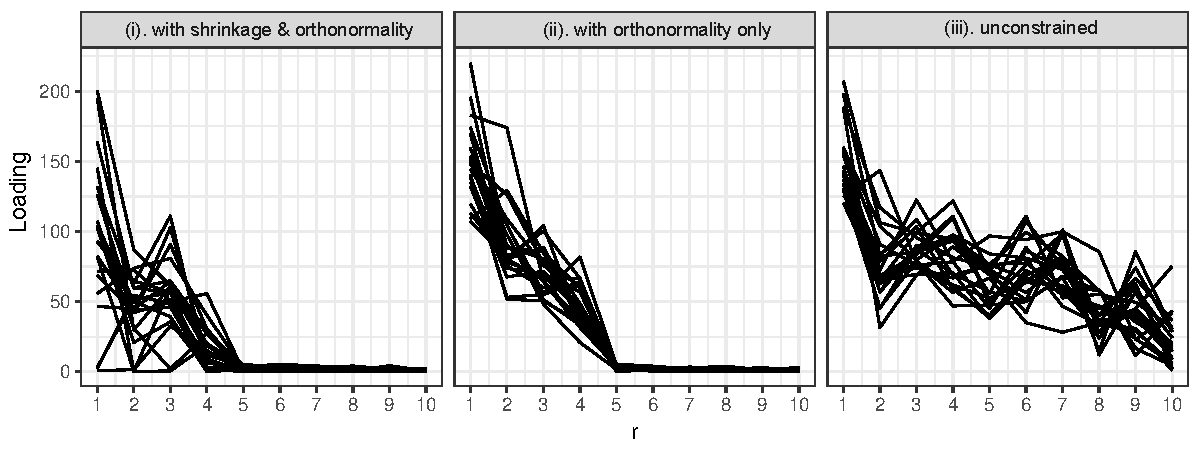
\includegraphics[width=1\textwidth]{network_loading}
		\caption{Posterior mean of the loadings $v_{i,r}$ for 21 subjects
			using three models. Each line represents the loadings for one
			subject over $r=1,\ldots10$.} \end{subfigure}
	\begin{subfigure}[b]{1\textwidth}
		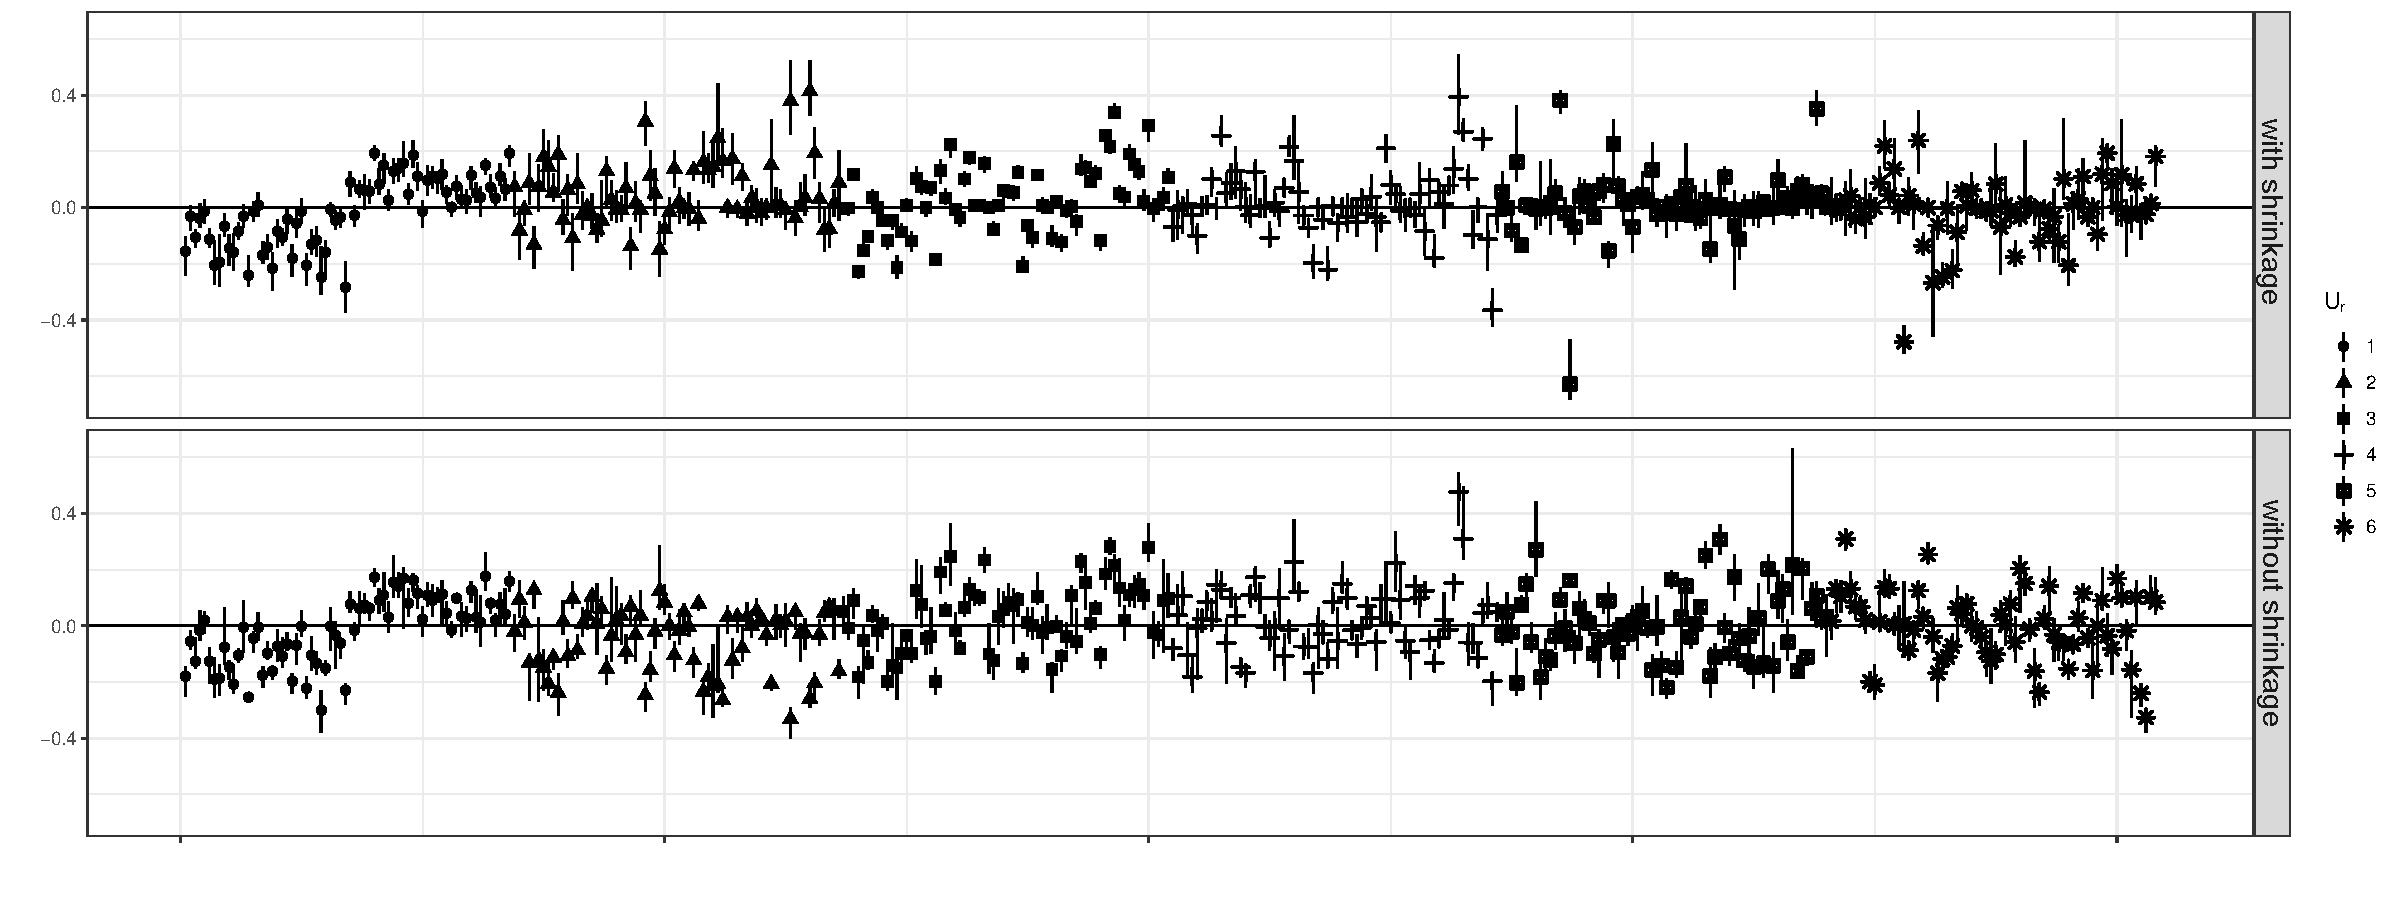
\includegraphics[width=1\textwidth]{network_factor.pdf}
		\caption{Posterior mean and pointwise $95\%$ credible interval of
			the factors $U_1,\ldots, U_6$ in the two constrained
			models. } \end{subfigure} \caption{Loadings and factors estimates
		of the network models. Panel (a) compares the varying loadings of
		the subjects in three models; Panel (b) compares the estimated
		shared factors with and without the shrinkage prior (model (iii) is
		omitted due to non-convergence in the factors).
		\label{network_model_basis}} \end{figure}




\section{Discussion}

Parameter constraint often limits the flexibility to develop new model and
creates huge burden in developing efficient posterior sampling algorithms.
In this article, we develop a formal strategy to utilize the large pool of
distributions in the constrained space, and propose a constraint relaxation
approach to allow simple implementation for posterior estimation. For
common constrained space that can be projected to via a function, we
propose an exact algorithm based on data augmentation; for more general
problem, we propose an approximation approach.  This strategy works well
for general equality and inequality constraints.


The future work of this research may include tackling the  `doubly
intractable' problem. This issue is common when the data is on the
constrained space, or the constrained prior has hyper-parameters to
estimate. In the data application, we show that a reparameterization
strategy works for some shrinkage priors, but clearly, more general
treatment is needed. We expect our work to be compatible to the existing
solutions \citep{murray2012mcmc,rao2016data, stoehr2017noisy}.

\appendix



\section{Proofs for Section 3.1}
\label{APP:Positive_Measure_Convergence_Proofs} \begin{proof}{Proof of
		Lemma \ref{THM:positive_measure_approximation_error}} \\ Recall,
	that the distance function $v_{\mc D}(\theta)$ is chosen so that
	$v_{\mc D}(\theta)$ is zero for all $\theta\in \mathcal{D}$. It follows
	that for any function $g$ \begin{equation} \begin{split}
			&\int_{\mathcal{R}}  g(\theta)
			\mathcal{L}(\theta;Y)\pi_\mathcal{R}(\theta)\exp(-v_{\mc D}(\theta)/\lambda)
			d\mu_\mathcal{R}(\theta) \\ &=  \int_{\mathcal{R}\setminus
				\mathcal{D}}g(\theta)
			\mathcal{L}(\theta;Y)\pi_\mathcal{R}(\theta)\exp(-v_{\mc D}(\theta)/\lambda)
			d\mu_\mathcal{R}(\theta) + \int_{ \mathcal{D}} g(\theta)
			\mathcal{L}(\theta;Y)\pi_\mathcal{R}(\theta)\exp(-v_{\mc D}(\theta)/\lambda)
			d\mu_\mathcal{R}(\theta) .  \end{split} \end{equation}

	Then, \begin{align*}  & \bigg|
		E[g(\theta)|\theta\in\mathcal{D}]-E_{\tilde{\pi}_\lambda}[g(\theta)]\bigg|
		\\ &= \bigg|\frac{ \int_\mathcal{D} g(\theta)
			\mathcal{L}(\theta;Y)\pi_\mathcal{R}(\theta)d\mu_\mathcal{R}(\theta)}{\int_\mathcal{D}
			\mathcal{L}(\theta;Y)\pi_\mathcal{R}(\theta)d\mu_\mathcal{R}(\theta)}
		- \frac{\int_{\mathcal{R}} g(\theta)
			\mathcal{L}(\theta;Y)\pi_\mathcal{R}(\theta)\exp\big(-v_{\mc D}(\theta)/\lambda)d\mu_\mathcal{R}(\theta)}{\int_{\mathcal{R}}
			\mathcal{L}(\theta;Y)\pi_\mathcal{R}(\theta)\exp\big(-v_{\mc D}(\theta)/\lambda)d\mu_\mathcal{R}(\theta)}
		\bigg|    \\ & =
		\bigg|\frac{\int_{\mathcal{R}\setminus
				\mathcal{D}}
			\mathcal{L}(\theta;Y)\pi_\mathcal{R}(\theta)\exp(-v_{\mc D}(\theta)/\lambda
			) d\mu_\mathcal{R}(\theta) \cdot \int_\mathcal{D}g(\theta)
			\mathcal{L}(\theta;Y)\pi_\mathcal{R}(\theta)d\mu_\mathcal{R}(\theta)-\int_\mathcal{D}\mathcal{L}(\theta;Y)\pi_\mathcal{R}(\theta)d\mu_\mathcal{R}(\theta)
			\cdot \int_{\mathcal{R}\setminus \mathcal{D} } g(\theta)
			\mathcal{L}(\theta;Y)\pi_\mathcal{R}(\theta)\exp(-v_{\mc D}(\theta)/\lambda)
			d\mu_\mathcal{R}(\theta)}{\int_\mathcal{D}
			\mathcal{L}(\theta;Y)\pi_\mathcal{R}(\theta)d\mu_\mathcal{R}(\theta)[\int_\mathcal{D}
				\mathcal{L}(\theta;Y)\pi_\mathcal{R}(\theta)d\mu_\mathcal{R}(\theta) +
				\int_{\mathcal{R}\setminus\mathcal{D}}
				\mathcal{L}(\theta;Y)\pi_\mathcal{R}(\theta) \exp(-v_{\mc D}(\theta)/\lambda)
				d\mu_\mathcal{R}(\theta)] }  \bigg|\end{align*} where the second equality
	follows from combining the fractions and making use of (3). We can bound
	the denominator from below by  $ \big[\int_\mathcal{D}
			\mathcal{L}(\theta;Y)\pi_\mathcal{R}(\theta) d\mu_\mathcal{R}(\theta)
			\big]^2>0$ so that

	\begin{equation*} \begin{split} &\big|
			E[g(\theta)|\theta\in\mathcal{D}]-E_{\tilde{\pi}_\lambda}[g(\theta)]\big|
			\\ &\le \frac{\big|\int_{\mathcal{R}\setminus \mathcal{D}}
				\mathcal{L}(\theta;Y)\pi_\mathcal{R}(\theta)\exp(-v_{\mc D}(\theta)/\lambda
				) d\mu_\mathcal{R}(\theta) \cdot \int_\mathcal{D}g(\theta)
				\mathcal{L}(\theta;Y)\pi_\mathcal{R}(\theta)d\mu_\mathcal{R}(\theta)
				-\int_\mathcal{D}\mathcal{L}(\theta;Y)\pi_\mathcal{R}(\theta)d\mu_\mathcal{R}(\theta)
				\cdot \int_{\mathcal{R}\setminus \mathcal{D} }
				g(\theta)\mathcal{L}(\theta;Y)\pi_\mathcal{R}(\theta)(z)\exp(-v_{\mc D}(\theta)/\lambda)
				d\mu_\mathcal{R}(\theta)\big|}{C_\mathcal{D}^2 } \end{split}
	\end{equation*} where $C_\mathcal{D} = \int_\mathcal{D}
		\mathcal{L}(\theta;Y)\pi_\mathcal{R}(\theta) d\mu_\mathcal{R}(\theta).$  If
	we add and subtract $$\int_{\mathcal{R}\setminus \mathcal{D}}
		\mathcal{L}(\theta;Y)\pi_\mathcal{R}(\theta)\exp(-v_{\mc D}(\theta)/\lambda )
		d\mu_\mathcal{R}(\theta) \cdot \int_{\mathcal{R}\setminus \mathcal{D}}
		g(\theta)
		\mathcal{L}(\theta;Y)\pi_\mathcal{R}(\theta)\exp(-v_{\mc D}(\theta)/\lambda )
		d\mu_\mathcal{R}(\theta)  $$ within the numerator, we can apply the
	triangle inequality. Thus,

	\begin{align*}  & \big|
		E[g(\theta)|\theta\in\mathcal{D}]-E_{\tilde{\pi}_\lambda}[g(\theta)]\big|
		\\ & \le \frac{ \bigg| \int_{\mathcal{R}\setminus \mathcal{D}}
			\mathcal{L}(\theta;Y)\pi_\mathcal{R}(\theta)\exp(-v_{\mc D}(\theta)/\lambda
			) d\mu_\mathcal{R}(\theta) \bigg| \cdot \bigg|\int_\mathcal{D}g(\theta)
			\mathcal{L}(\theta;Y)\pi_\mathcal{R}(\theta)d\mu_\mathcal{R}(\theta) -
			\int_{\mathcal{R}\setminus \mathcal{D}} g(\theta)
			\mathcal{L}(\theta;Y)\pi_\mathcal{R}(\theta)\exp(-v_{\mc D}(\theta)/\lambda )
			d\mu_\mathcal{R}(\theta)  \bigg|}{C_\mathcal{D}^2 }\dots \\ &
		\hspace{0.5cm} + \frac{\bigg| \int_{\mathcal{R}\setminus \mathcal{D}}
			g(\theta)
			\mathcal{L}(\theta;Y)\pi_\mathcal{R}(\theta)\exp(-v_{\mc D}(\theta)/\lambda )
			d\mu_\mathcal{R}(\theta) \bigg| \cdot \bigg|\int_\mathcal{D}
			\mathcal{L}(\theta;Y)\pi_\mathcal{R}(\theta)d\mu_\mathcal{R}(\theta)-
			\int_{\mathcal{R}\setminus \mathcal{D}}
			\mathcal{L}(\theta;Y)\pi_\mathcal{R}(\theta)\exp(-v_{\mc D}(\theta)/\lambda )
			d\mu_\mathcal{R}(\theta)  \bigg|}{C_\mathcal{D}^2 }\end{align*} Since
	$g\in\mathbb{L}^1(\mathcal{R},\mathcal{L}(\theta;Y)\pi_\mathcal{R}d\mu_\mathcal{R})$,
	we can then bound the numerators as follows.  First, \begin{align*}  & \bigg|
		\int_{\mathcal{R}\setminus \mathcal{D}}
		\mathcal{L}(\theta;Y)\pi_\mathcal{R}(\theta)\exp(-v_{\mc D}(\theta)/\lambda
		) d\mu_\mathcal{R}(\theta) \bigg| \cdot \bigg|\int_\mathcal{D}
		g(y_i)
		\mathcal{L}(\theta;Y)\pi_\mathcal{R}(\theta)d\mu_\mathcal{R}(\theta)
		- \int_{\mathcal{R}\setminus \mathcal{D}} g(\theta)
		\mathcal{L}(\theta;Y)\pi_\mathcal{R}(\theta)\exp(-v_{\mc D}(\theta)/\lambda
		)d\mu_\mathcal{R}(\theta) \bigg|       \\ & \le \bigg|
		\int_{\mathcal{R}\setminus \mathcal{D}}
		\mathcal{L}(\theta;Y)\pi_\mathcal{R}(\theta)\exp(-v_{\mc D}(\theta)/\lambda
		) d\mu_\mathcal{R}(\theta) \bigg| \cdot \bigg( \bigg|
		\int_\mathcal{D}g(\theta)
		\mathcal{L}(\theta;Y)\pi_\mathcal{R}(\theta)d\mu_\mathcal{R}(\theta) \bigg|
		+ \bigg| \int_{\mathcal{R}\setminus \mathcal{D}} g(\theta)
		\mathcal{L}(\theta;Y)\pi_\mathcal{R}(\theta)\exp(-v_{\mc D}(\theta)/\lambda )
		d\mu_\mathcal{R}(\theta) \bigg| \bigg) \\ &\le \int_{\mathcal{R}\setminus
			\mathcal{D}}
		\mathcal{L}(\theta;Y)\pi_\mathcal{R}(\theta)\exp(-v_{\mc D}(\theta)/\lambda )
		d\mu_\mathcal{R}(\theta)  \cdot \bigg(\int_\mathcal{D}|g(y_i)|
		\mathcal{L}(\theta;Y)\pi_\mathcal{R}(\theta)d\mu_\mathcal{R}(\theta)  +
		\int_{\mathcal{R}\setminus \mathcal{D}} |g(\theta)|
		\mathcal{L}(\theta;Y)\pi_\mathcal{R}(\theta)\exp(-v_{\mc D}(\theta)/\lambda )
		d\mu_\mathcal{R}(\theta)  \bigg)       \\ &\le \int_{\mathcal{R}\setminus
			\mathcal{D}}
		\mathcal{L}(\theta;Y)\pi_\mathcal{R}(\theta)\exp(-v_{\mc D}(\theta)/\lambda )
		d\mu_\mathcal{R}(\theta)  \cdot  \int_{\mathcal{R}} |g(x_i)|
		\mathcal{L}(\theta;Y)\pi_\mathcal{R}(\theta) d\mu_\mathcal{R}(\theta)   =
		C_\mathcal{R} E|g(x_i)| \int_{\mathcal{R}\setminus \mathcal{D}}
		\mathcal{L}(\theta;Y)\pi_\mathcal{R}(\theta)\exp(-v_{\mc D}(\theta)/\lambda )
		d\mu_\mathcal{R}(\theta).\end{align*} Here, $C_\mathcal{R} =
		\int_\mathcal{R}
		\mathcal{L}(\theta;Y)\pi_\mathcal{R}(\theta)d\mu_\mathcal{R}(\theta)$ is
	the normalizing constant of $\mathcal{L}(\theta;Y)\pi_\mathcal{R}.$
	Secondly, \begin{align*}  & \bigg| \int_{\mathcal{R}\setminus \mathcal{D}}
		g(\theta)
		\mathcal{L}(\theta;Y)\pi_\mathcal{R}(\theta)\exp(-v_{\mc D}(\theta)/\lambda
		) d\mu_\mathcal{R}(\theta) \bigg| \cdot \bigg|\int_\mathcal{D}
		\mathcal{L}(\theta;Y)\pi_\mathcal{R}(\theta)d\mu_\mathcal{R}(\theta)
		- \int_{\mathcal{R}\setminus \mathcal{D}}
		\mathcal{L}(\theta;Y)\pi_\mathcal{R}(\theta)\exp(-v_{\mc D}(\theta)/\lambda
		) d\mu_\mathcal{R}(\theta)  \bigg|                \\ & \le
		\int_{\mathcal{R}\setminus \mathcal{D}} |g(\theta)|
		\mathcal{L}(\theta;Y)\pi_\mathcal{R}(\theta)\exp(-v_{\mc D}(\theta)/\lambda
		) dx  \cdot \bigg|\int_\mathcal{D}
		\mathcal{L}(\theta;Y)\pi_\mathcal{R}(\theta)d\mu_\mathcal{R}(\theta)
		\bigg| + \bigg| \int_{\mathcal{R}\setminus \mathcal{D}}
		\mathcal{L}(\theta;Y)\pi_\mathcal{R}(\theta)\exp(-v_{\mc D}(\theta)/\lambda
		) d\mu_\mathcal{R}(\theta) \bigg|                 \\ &\le
		\int_{\mathcal{R}\setminus \mathcal{D}} |g(\theta)|
		\mathcal{L}(\theta;Y)\pi_\mathcal{R}(\theta)\exp(-v_{\mc D}(\theta)/\lambda
		) d\mu_\mathcal{R}(\theta) \bigg(\int_\mathcal{D}
		\mathcal{L}(\theta;Y)\pi_\mathcal{R}(\theta)d\mu_\mathcal{R}(\theta)
		+  \int_{\mathcal{R}\setminus \mathcal{D}}
		\mathcal{L}(\theta;Y)\pi_\mathcal{R}(\theta) d\mu_\mathcal{R}(\theta)
		\bigg)                                            \\ & = \int_{\mathcal{R}\setminus \mathcal{D}} |g(\theta)|
		\mathcal{L}(\theta;Y)\pi_\mathcal{R}(\theta)\exp(-v_{\mc D}(\theta)/\lambda )
		d\mu_\mathcal{R}(\theta).\end{align*} Thus, we have the bounds specified
	by the theorem, \begin{align*}  & \big|
		E[g(\theta)|\theta\in\mathcal{D}]-E_{\tilde{\pi}_\lambda}[g(\theta)]\big|
		\\ & \le \frac{C_\mathcal{R}E|g(\theta)| \int_{\mathcal{R}\setminus
				\mathcal{D}}
			\mathcal{L}(\theta;Y)\pi_\mathcal{R}(\theta)\exp(-v_{\mc D}(\theta)/\lambda )
			d\mu_\mathcal{R}(\theta)}{C_\mathcal{D}^2 } +
		\frac{\int_{\mathcal{R}\setminus \mathcal{D}} |g(\theta)|
			\mathcal{L}(\theta;Y)\pi_\mathcal{R}(\theta)\exp(-v_{\mc D}(\theta)/\lambda )
			d\mu_\mathcal{R}(\theta)}{C_\mathcal{D}^2 } \\ &=
		\frac{\int_{\mathcal{R}\setminus \mathcal{D}}
		(C_\mathcal{R}E|g(\theta)|+|g(\theta)|)
		\mathcal{L}(\theta;Y)\pi_\mathcal{R}(\theta)\exp(-v_{\mc D}(\theta)/\lambda )
		d\mu_\mathcal{R}(\theta)}{C_\mathcal{D}^2 }.\end{align*}

	It remains to be shown that $$\big|
		E[g(\theta)|\theta\in\mathcal{D}]-E_{\tilde{\pi}_\lambda}[g(\theta)]\big|
		\to 0 \text{ as }\lambda\to0^+.$$ Again, by the assumptions that
	$g\in\mathbb{L}^1(\mathcal{R},\mathcal{L}(\theta;Y)\pi_\mathcal{R}d\mu_\mathcal{R})$
	and $v_{\mc D}(\theta) >0$ for $\mu_\mathcal{R}$ a.e.  $\theta \in
		\mathcal{R}\setminus \mathcal{D}$, it follows that
	$(C_\mathcal{R}E|g(x_i)|+|g(x_i)|)
		\mathcal{L}(\theta;Y)\pi_\mathcal{R}(\theta)$ is a dominating function of
	$(C_\mathcal{R}E|g(x_i)|+|g(x_i)|)
		\mathcal{L}(\theta;Y)\pi_\mathcal{R}(\theta)\exp(-v_{\mc D}(\theta)/\lambda )$
	which converges to zero for $\mu_\mathcal{R}$-a.e.
	$\theta\in\mathcal{R}\setminus\mathcal{D}$ as $\lambda\to 0^+.$ Thus, by
	the dominated convergence theorem, $\big|
		E[g(\theta)|\theta\in\mathcal{D}]-E_{\tilde{\pi}_\lambda}[g(\theta)]\big|\to
		0$ as $\lambda\to0^+.$

\end{proof}


\begin{proof}{Proof of Theorem \ref{THM:Positive_measure_convergence_rate}}
	\\

	We begin with the bound from Lemma
	\ref{THM:positive_measure_approximation_error}.  $$\big|
		E[g(\theta)|\theta\in\mathcal{D}]-E_{\tilde{\pi}_\lambda}[g(\theta)]\big|
		\le \frac{\int_{\mathcal{R}\setminus \mathcal{D}}
		(C_\mathcal{R}E|g(\theta)|+|g(\theta)|)
		\mathcal{L}(\theta;Y)\pi_\mathcal{R}(\theta)\exp(-v_{\mc D}(\theta)/\lambda )
		d\mu_\mathcal{R}(\theta)}{C_\mathcal{D}^2 }.$$ For the moment, let us focus
	on the numerator of the previous expression.  By the Cauchy-Schwartz
	inequality, \begin{align*}  & \int_{\mathcal{R}\setminus \mathcal{D}}
		(C_\mathcal{R}E|g(\theta)|+|g(\theta)|)
		\mathcal{L}(\theta;Y)\pi_\mathcal{R}(\theta)\exp(-v_{\mc D}(\theta)/\lambda
		) d\mu_\mathcal{R}(\theta)                 \\ &\le \bigg(\int_{\mathcal{R}\setminus
		\mathcal{D}}   (C_\mathcal{R}E|g(\theta)|+|g(\theta)|)^2
		\mathcal{L}(\theta;Y)\pi_\mathcal{R}(\theta)d\mu_\mathcal{R}(\theta)\bigg)^{1/2}
		\bigg(\int_{\mathcal{R}\setminus \mathcal{D}}\exp(-2v_{\mc D}(\theta)/\lambda
		)\mathcal{L}(\theta;Y)\pi_\mathcal{R}(\theta)
		d\mu_\mathcal{R}(\theta)\bigg)^{1/2}       \\ &\le \bigg(\int_{\mathcal{R}}
		(C_\mathcal{R}E|g(\theta)|+|g(\theta)|)^2
		\mathcal{L}(\theta;Y)\pi_\mathcal{R}(\theta)d\mu_\mathcal{R}(\theta)\bigg)^{1/2}
		\bigg(\int_{\mathcal{R}\setminus \mathcal{D}}\exp(-2v_{\mc D}(\theta)/\lambda
		)\mathcal{L}(\theta;Y)\pi_\mathcal{R}(\theta)
		d\mu_\mathcal{R}(\theta)\bigg)^{1/2}\end{align*} By assumption,
	$g\in\mathbb{L}^2(\mathcal{R},\mathcal{L}(\theta;Y)\pi_\mathcal{R}\mu_\mathcal{R}).$
	Thus, \begin{align*}  & \int_{\mathcal{R}\setminus \mathcal{D}}
		(C_\mathcal{R}E|g(\theta)|+|g(\theta)|)
		\mathcal{L}(\theta;Y)\pi_\mathcal{R}(\theta)\exp(-v_{\mc D}(\theta)/\lambda
		) d\mu_\mathcal{R}(\theta)                                         \\
		 & =\underbrace{\bigg([C_\mathcal{R}^3+2C_\mathcal{R}^2](E|g|)^2 +
		C_\mathcal{R}E[|g|^2]
		\bigg)^{1/2}}_{C_{\mathcal{R},g}<\infty}\bigg(\int_{\mathcal{R}\setminus
			\mathcal{D}}\exp(-2v_{\mc D}(\theta)/\lambda
		)\mathcal{L}(\theta;Y)\pi_\mathcal{R}(\theta)
		d\mu_\mathcal{R}(\theta)\bigg)^{1/2}                               \\
		 & =C_{\mathcal{R},g}\bigg(\int_{\mathcal{R}\setminus
			\mathcal{D}}\exp(-2v_{\mc D}(\theta)/\lambda
		)\mathcal{L}(\theta;Y)\pi_\mathcal{R}(\theta)
		d\mu_\mathcal{R}(\theta)\bigg)^{1/2}\end{align*} We separate the integral
	$$\int_{\mathcal{R}\setminus \mathcal{D}}\exp(-2v_{\mc D}(\theta)/\lambda
		)\mathcal{L}(\theta;Y)\pi_\mathcal{R}(\theta) d\mu_\mathcal{R}(\theta)$$
	over the sets $\{\theta: v_{\mc D}(\theta)> -\lambda\log\lambda\}$ and $\{\theta:
		\, 0< v_{\mc D}(\theta)< -\lambda\log\lambda\}.$ \begin{align*}
		 & \int_{\mathcal{R}\setminus \mathcal{D}}\exp(-2v_{\mc D}(\theta)/\lambda
		)\mathcal{L}(\theta;Y)\pi_\mathcal{R}(\theta)
		d\mu_\mathcal{R}(\theta)                                             \\ &= \int_{\{\theta: v_{\mc D}(\theta)>
			-\lambda\log\lambda\}}\exp(-2v_{\mc D}(\theta)/\lambda
		)\mathcal{L}(\theta;Y)\pi_\mathcal{R}(\theta)
		d\mu_\mathcal{R}(\theta) +\int_{\{\theta: \,0 < v_{\mc D}(\theta)<
			-\lambda\log\lambda\}}\exp(-2v_{\mc D}(\theta)/\lambda
		)\mathcal{L}(\theta;Y)\pi_\mathcal{R}(\theta)
		d\mu_\mathcal{R}(\theta)                                             \\ &\le \lambda^2 \int_{\{\theta:
			v_{\mc D}(\theta)>
			-\lambda\log\lambda\}}\mathcal{L}(\theta;Y)\pi_\mathcal{R}(\theta)
		d\mu_\mathcal{R}(\theta)+\int_{\{\theta: \,0< v_{\mc D}(\theta)<
			-\lambda\log\lambda\}}\exp(-2v_{\mc D}(\theta)/\lambda
		)\mathcal{L}(\theta;Y)\pi_\mathcal{R}(\theta)
		d\mu_\mathcal{R}(\theta)                                             \\ &\le C_\mathcal{R}\lambda^2
		+\int_{\{\theta: \, 0< v_{\mc D}(\theta)<
			-\lambda\log\lambda\}}\exp(-2v_{\mc D}(\theta)/\lambda
		)\mathcal{L}(\theta;Y)\pi_\mathcal{R}(\theta) d\mu_\mathcal{R}(\theta)
	\end{align*} To review, to this point we have shown that \begin{equation}
		\big|
		E[g(\theta)|\theta\in\mathcal{D}]-E_{\tilde{\pi}_\lambda}[g(\theta)]\big|
		\le
		\frac{C_{\mathcal{R},g}}{D_\mathcal{D}^2}\bigg(C_\mathcal{R}\lambda^2
		+ \int_{\{\theta: \, 0< v_{\mc D}(\theta)<
			-\lambda\log\lambda\}}\exp(-2v_{\mc D}(\theta)/\lambda
		)\mathcal{L}(\theta;Y)\pi_\mathcal{R}(\theta) d\mu_\mathcal{R}(\theta)
		\bigg)^{1/2} \end{equation} From the requirements of Theorem
	\ref{THM:Positive_measure_convergence_rate}, we now let $v_{\mc D}(\theta) =
		\inf_{x\in \mathcal{D}}\|\theta - x\|_2$ and assume that $\mathcal{D}$ has
	a piecewise smooth boundary.  In this case, the set $\{\theta: \,0 <
		v_{\mc D}(\theta)< -\lambda\log\lambda\}$ forms a `shell' of thickness $-\lambda
		\log \lambda$ which encases $\mathcal{D}.$

	For the moment, suppose that $\mathcal{D}$ is a bounded subset of
	$\mathcal{R}$. Furthermore, suppose we take $\lambda$ sufficiently small so
	that $\mathcal{L}(\theta;Y)\pi_\mathcal{R}(\theta)$ is continuous on
	$V_\lambda = \{\theta: \,0 < v_{\mc D}(\theta)< -\lambda\log\lambda\}.$ Observe
	that  \begin{align*}  & \int\limits_{\{\theta: \, 0< v_{\mc D}(\theta)<
			-\lambda\log\lambda\}}\exp(-2v_{\mc D}(\theta)/\lambda
		)\mathcal{L}(\theta;Y)\pi_\mathcal{R}(\theta)
		d\mu_\mathcal{R}(\theta)  \le
		\sup_{V_\lambda}|\mathcal{L}(\theta;Y)\pi_\mathcal{R}(\theta)|
		\int_{V\lambda}\exp(-2v_{\mc D}(\theta)/\lambda ) d\mu_{R}(\theta) \\ &
		\le \sup_{V_\lambda}|\mathcal{L}(\theta;Y)\pi_\mathcal{R}(\theta)|
		\int_{V\lambda} d\mu_{R}(\theta)=
		\sup_{V_\lambda}|\mathcal{L}(\theta;Y)\pi_\mathcal{R}(\theta)|
		\cdot Vol(V_\lambda)                                         \\ &=
		\sup_{V_\lambda}|\mathcal{L}(\theta;Y)\pi_\mathcal{R}(\theta)|
		S_\mathcal{D} \cdot \lambda |\log \lambda|\end{align*}  Here,$
		S_\mathcal{D}$ is the surface area of boundary of $\mathcal{D}$, which is
	finite by the assumptions that $\mathcal{D}$ is bounded and has a piecewise
	smooth boundary. Additionally, since $V_\lambda$ is relatively compact, it
	follows that
	$\sup_{V_\lambda}|\mathcal{L}(\theta;Y)\pi_\mathcal{R}(\theta)| < \infty.$

	Consider the more general case where $\mathcal{D}$ is not a bounded subset
	of $\mathcal{R}.$ Since
	$\int_\mathcal{R}\mathcal{L}(\theta;Y)\pi_\mathcal{R}(\theta)d\mu_\mathcal{R}(\theta)$,
	there exists a radius $\rho$ such that $\int_{\|\theta\|_2 >
			\rho}\mathcal{L}(\theta;Y)\pi_\mathcal{R}(\theta)d\mu_\mathcal{R}(\theta)<
		\lambda^2.$  Note that, for $\theta \in V_\lambda$,
	$J(v_{\mc D}(\theta))=\sqrt{(Dv_{\mc D})'(Dv_{\mc D})} = 2.$ By the co-area formula
	\cite{diaconis2013manifold,federer2014geometric} $$\int\limits_{\{\theta:
			\, 0< v_{\mc D}(\theta)< -\lambda\log\lambda\}}\exp(-2v_{\mc D}(\theta)/\lambda
		)\mathcal{L}(\theta;Y)\pi_\mathcal{R}(\theta) d\mu_\mathcal{R}(\theta)  =
		\int_0^{-\lambda\log\lambda} e^{-\frac{x}{\lambda}}\bigg(
		\int_{v_{\mc D}^{-1}(x)} \frac{1}{2}\mathcal{L}(\theta;Y) \pi_\mathcal{R}(\theta)
		d\bar{\mathcal{H}}^{r-1}(\theta)\bigg) dx$$ Again, we may take $\lambda$
	sufficiently small so that $\mathcal{L}(\theta;Y) \pi_\mathcal{R}(\theta) $
	is continuous on $V_\lambda.$  As such, the function $ \int_{v_{\mc D}^{-1}(x)}
		\frac{1}{2}\mathcal{L}(\theta;Y) \pi_\mathcal{R}(\theta)
		d\bar{\mathcal{H}}^{r-1}(\theta)$ is a continuous map from the closed
	interval, $[0,-\lambda\log\lambda]$, to $\mathbb{R}.$ Hence it is bounded.
	As a result, \begin{align*}  & \int\limits_{\{\theta: \, 0< v_{\mc D}(\theta)<
			-\lambda\log\lambda\}}\exp(-2v_{\mc D}(\theta)/\lambda
		)\mathcal{L}(\theta;Y)\pi_\mathcal{R}(\theta)
		d\mu_\mathcal{R}(\theta)                     \\ &\le \sup_{x \in
			[0,-\lambda\log\lambda]} \bigg( \int_{v_{\mc D}^{-1}(x)}
		\frac{1}{2}\mathcal{L}(\theta;Y) \pi_\mathcal{R}(\theta)
		d\bar{\mathcal{H}}^{r-1}(\theta)\bigg) \cdot \int_0^{-\lambda\log \lambda}
		e^{-\frac{x}{\lambda}}dx                     \\ & = \sup_{x \in [0,-\lambda\log\lambda]} \bigg(
		\int_{v_{\mc D}^{-1}(x)} \frac{1}{2}\mathcal{L}(\theta;Y) \pi_\mathcal{R}(\theta)
		d\bar{\mathcal{H}}^{r-1}(\theta)\bigg)  \cdot (\lambda - \lambda^2) =
		O(\lambda)\end{align*} This result also applies to the case where
	$\mathcal{D}$ is bounded.  Thus, we may conclude that \begin{align*}  & \big|
		E[g(\theta)|\theta\in\mathcal{D}]-E_{\tilde{\pi}_\lambda}[g(\theta)]\big| \\
		 & \le
		\frac{C_{\mathcal{R},g}}{D_\mathcal{D}^2}\bigg(C_\mathcal{R}\lambda^2
		+ \sup_{x \in [0,-\lambda\log\lambda]} \bigg( \int_{v_{\mc D}^{-1}(x)}
		\frac{1}{2}\mathcal{L}(\theta;Y) \pi_\mathcal{R}(\theta)
		d\bar{\mathcal{H}}^{r-1}(\theta)\bigg)  \cdot (\lambda - \lambda^2)
		\bigg)^{1/2}                                                              \\ &= \frac{C_{\mathcal{R},g}}{D_\mathcal{D}^2} \cdot \sup_{x
			\in [0,-\lambda\log\lambda]} \bigg( \int_{v_{\mc D}^{-1}(x)}
		\frac{1}{2}\mathcal{L}(\theta;Y) \pi_\mathcal{R}(\theta)
		d\bar{\mathcal{H}}^{r-1}(\theta)\bigg)  \cdot \sqrt{\lambda} +
		o(\sqrt{\lambda})\end{align*} Since $\sup_{x \in [0,-\lambda\log\lambda]}
		\bigg( \int_{v_{\mc D}^{-1}(x)} \frac{1}{2}\mathcal{L}(\theta;Y)
		\pi_\mathcal{R}(\theta) d\bar{\mathcal{H}}^{r-1}(\theta)\bigg)$ is a
	decreasing function in $\lambda$, we may conclude that $\big|
		E[g(\theta)|\theta\in\mathcal{D}]-E_{\tilde{\pi}_\lambda}[g(\theta)]\big| =
		O(\sqrt{\lambda}).$ \end{proof}

\section{Proofs from Section 3.2}

\begin{proof} Recall that we have two densities. The first is the fully
	constrained density for $\theta\in\mathcal{D}$.  \begin{equation*}
		\pi_\mathcal{D}(\theta) = \frac{1}{m_0}
		\frac{\mathcal{L}(y;\theta)\pi_\mathcal{R}(\theta)}{J(\nu(\theta))}\mathbbm{1}_\mathcal{D}(\theta)
	\end{equation*} where the normalizing constant $m_0$ is calculated
	w.r.t. Hausdorff measure $$m_0 = \int_\mathcal{R}
		\frac{\mathcal{L}(y;\theta)\pi_\mathcal{R}(\theta)}{J(\nu(\theta))}\mathbbm{1}_\mathcal{D}(\theta)d\bar{\mathcal{H}}^{r-s}(\theta).$$
	%This density defines a probability measure, $\Pi$, w.r.t. Hausdorff
	%measure.  For a measurable set $E$, $$\Pi(E) = \int_E
	%\frac{g(\theta)}{m_0}
	%\frac{\mathcal{L}(y;\theta)\pi_\mathcal{R}(\theta)}{J(\nu(\theta))}\mathbbm{1}_\mathcal{D}(\theta)d\bar{\mathcal{H}}^{r-s}(\theta).$$

	Secondly, we have the relaxed distribution
	$$\tilde{\pi}_\mathcal{D}(\theta) = \frac{1}{m_\lambda}
		\mathcal{L}(y;\theta)\pi_\mathcal{R}(\theta)\exp\bigg(-\frac{\|v(\theta)\|_1}{\lambda}\bigg)$$
	where the normalizing constant is calculated w.r.t. Lebesgue measure on
	$\mathcal{R}$, denote by $\mu_\mathcal{R}$, $$m_\lambda =
		\int_\mathcal{R}\mathcal{L}(y;\theta)\pi_\mathcal{R}(\theta)\exp\bigg(-\frac{\|v(\theta)\|_1}{\lambda}\bigg)
		d\mu_\mathcal{R}(\theta).$$
	%We use $\mu_\mathcal{R}$ to denote Lebesgue measure on $\mathcal{R}.$ This
	%density defines a probability measure, $\tilde{\Pi}$, w.r.t.
	%$\mu_\mathcal{R}$.  For a measurable set $E$, $$\tilde{\Pi}(E) = \int_E
	%\frac{g(\theta)}{m_\lambda}
	%\mathcal{L}(y;\theta)\pi_\mathcal{R}(\theta)\exp\bigg(-\frac{\|v(\theta)\|_1}{\lambda}\bigg)d\mu_\mathcal{R}(\theta).$$

	%\noindent \textbf{Definition of expectation of $g(\theta)$ w.r.t.
	%constrained and relaxed measures}

	For a given function, $g:\mathcal{R}\to\mathbb{R}$, we can define the exact
	and approximate expectations of $g$, respectively $E_\Pi$ and
	$E_{\tilde{\Pi}}$, as \begin{align*} E_\Pi[g(\theta)]           & =
		E[g(\theta)|\theta\in\mathcal{D}] = \int_\mathcal{R}
		\frac{g(\theta)}{m_0}
		\frac{\mathcal{L}(y;\theta)\pi_\mathcal{R}(\theta)}{J(\nu(\theta))}\mathbbm{1}_\mathcal{D}(\theta)d\bar{\mathcal{H}}^{r-s}(\theta)
		\\ &=\int_\mathcal{D} \frac{g(\theta)}{m_0}
		\frac{\mathcal{L}(y;\theta)\pi_\mathcal{R}(\theta)}{J(\nu(\theta))}d\bar{\mathcal{H}}^{r-s}(\theta) \\
		E_{\tilde{\Pi}}[g(\theta)] & = \int_\mathcal{R}
		\frac{g(\theta)}{m_\lambda}
		\mathcal{L}(y;\theta)\pi_\mathcal{R}(\theta)\exp\bigg(-\frac{\|v(\theta)\|_1}{\lambda}\bigg)d\mu_\mathcal{R}(\theta)
		\\ &= \int_{\mathbb{R}^s} \frac{1}{m_\lambda} \int_{\nu^{-1}(x)}
		g(\theta)
		\frac{\pi_\mathcal{R}(\theta)\mathcal{L}(y;\theta)}{J(\nu(\theta))}
		\exp\bigg(-\frac{\|\nu(\theta)\|_1}{\lambda}\bigg)
		d\bar{\mathcal{H}}^{r-s}(\theta) d\mu_{\mathbb{R}^s}                                                \\
		                           & =\int_{\mathbb{R}^s}
		\frac{\exp\bigg(-\frac{\|x\|_1}{\lambda}\bigg) }{m_\lambda}
		\int_{\nu^{-1}(x)} g(\theta)
		\frac{\pi_\mathcal{R}(\theta)\mathcal{L}(y;\theta)}{J(\nu(\theta))}
		d\bar{\mathcal{H}}^{r-s}(\theta) d\mu_{\mathbb{R}^s}\end{align*}
	Let, $$m(x) = m^{r-s}(x) =
		\int_{\nu^{-1}(x)}\frac{\pi_\mathcal{R}(\theta)\mathcal{L}(y;\theta)}{J(\nu(\theta))}
		d\bar{\mathcal{H}}^{r-s}(\theta) .$$ By construction, $m(x) > 0$
	for $\mu_{\mathbb{R}^s}$-a.e. $x\in Range(\nu)$. In particular,
	$m_0=m(0)>0$. By Theorem 1, \begin{equation} E[g(\theta) |
		\nu(\theta) = x] = \frac{1}{m(x)} \int_{\nu^{-1}(x)}
		g(\theta)\frac{\pi_\mathcal{R}(\theta)\mathcal{L}(y;\theta)}{J(\nu(\theta))}
		d\bar{\mathcal{H}}^{r-s}(\theta).  \end{equation} As such, we may may
	express $E_{\tilde{\Pi}}[g(\theta)]$ as \begin{equation}
		E_{\tilde{\Pi}}[g(\theta)] = \int_{\mathbb{R}^s}
		\frac{m(x)}{m_\lambda}\exp\bigg(-\frac{\|x\|_1}{\lambda}\bigg)
		E\big[g(\theta)|\nu(\theta)=x\big] d\mu_{\mathbb{R}^s}(x).
	\end{equation}
	%To show $\tilde{E}[g(\theta)] \to E[g(\theta)|\nu(\theta)=0] =
	%E[g(\theta)|\theta\in\mathcal{D}]$ as $\lambda \to 0^+$, we first need to
	%investigate the behavior of $m_\lambda$ for $0<\lambda \ll 1.$

	%\begin{center}\line(1,0){450}\end{center}
	%
	%At this point, I'm going to try to demonstrate the asymptotic behavior of
	%(2) for small $\lambda.$ To write this up properly, we'll need to begin
	%with absolute values of differences and bound above. This will require
	%some statements about the integrability of $g$. I'm going to wait on
	%writing the argument up in that manner until we determine what can be said
	%about the continuity/uniform continuity/differentiability of $m$ and
	%$E[g|\nu=x]$ near $x=0.$ For now, I'll make the following assumptions.\\
	%
	%\noindent\textbf{Assumption:} Both $m$ and
	%$E\big[g(\theta)|\nu(\theta)=x\big]$ are continuous at $x=0.$
	%
	%\begin{center}\line(1,0){450}\end{center} \vspace{0.5cm} \noindent
	%\textbf{Asymptotic behavior of $m_\lambda$} \\
	%
	%\noindent Fix $\epsilon >0$. Since $-\lambda\log(\lambda^{s+1}) \to 0$ as
	%$\lambda\to 0^+$, we may choose $\lambda$ small enough so that
	%$\|m-m(0)\|_1 < \epsilon$ for all $x\in
	%B_1(0;\lambda|\log(\lambda^{s+1}|)$ and $\lambda <
	%\max(\epsilon^{1/s},\epsilon^{1/(s+1)})$, the 1-ball of radius
	%$\lambda|\log(\lambda^{s+1})|$ centered at $0.$ 
	%
	Let us first consider the small $\lambda$ behavior of $m_\lambda.$ We begin
	by re-expressing $m_\lambda$ in terms of $m(x)$ through the co-area
	formula.  \begin{align*} m_\lambda & = \int_\mathcal{R}
		\pi_\mathcal{R}(\theta) \mathcal{L}(y;\theta)
		\exp\bigg(-\frac{\|v(\theta)\|_1}{\lambda}\bigg)
		d\mu_\mathcal{R}(\theta)                                 \\ &= \int_{\mathbb{R}^s}
		\exp\bigg(-\frac{\|x\|_1}{\lambda}\bigg) \int_{\nu^{-1}(x)}
		\frac{\pi_\mathcal{R}(\theta)
			\mathcal{L}(y;\theta)}{J(\nu(\theta))}
		d\bar{\mathcal{H}}^{r-s}(\theta) d\mu_{\mathbb{R}^s} (x) \\
		          & =\int_{\mathbb{R}^s}m(x)
		\exp\bigg(-\frac{\|x\|_1}{\lambda}\bigg)d\mu_{\mathbb{R}^s}(x)\end{align*}

	Split the above integral into two regions: the interior and exterior of
	$B_1(0;\lambda|\log(\lambda^{s+1})|)$. Note that outside of $B_1$,
	$\exp(-\|x\|_1/\lambda) \le \lambda^{s+1}.$ \begin{align*} m_\lambda & =
		\int_{\mathbb{R}^s \setminus
			B_1(0;\lambda|\log(\lambda^{s+1})|)}m(x)
		\exp\bigg(-\frac{\|x\|_1}{\lambda}\bigg)d\mu_{\mathbb{R}^s}(x) +
		\int_{B_1(0;\lambda|\log(\lambda^{s+1})|)}m(x)
		\exp\bigg(-\frac{\|x\|_1}{\lambda}\bigg)d\mu_{\mathbb{R}^s}(x)            \\
		          & =O\bigg( \lambda^{s+1} \int_{\mathbb{R}^s \setminus
			B_1(0;\lambda|\log(\lambda^{s+1})|)}m(x)
		d\mu_{\mathbb{R}^s}(x)\bigg)                                              \\ &\hspace{2cm}+
		\int_{B_1(0;\lambda|\log(\lambda^{s+1})|)} m(x)
		\bigg[1+O\bigg(\frac{1}{\lambda}\exp\bigg(-\frac{\|x\|_1}{\lambda}\bigg)\bigg)\bigg]d\mu_{\mathbb{R}^s}(x)
		\\ &=O\bigg( \lambda^{s+1} \int_{\mathbb{R}^s \setminus
			B_1(0;\lambda|\log(\lambda^{s+1})|)}m(x) d\mu_{\mathbb{R}^s}(x)\bigg)     \\
		          & \hspace{2cm}+ \int_{B_1(0;\lambda|\log(\lambda^{s+1})|)} m(x)
		\bigg[1+O(\lambda^s) \bigg]d\mu_{\mathbb{R}^s}(x)\end{align*} Since $m(x)$
	is continuous on an open neighborhood containing the origin, we may choose
	$\lambda$ small enough so that $m(x)$ is uniformly continuous on
	$B_1(0;\lambda |\log \lambda^{s+1}|).$ Then, \begin{align*} m_\lambda & =
		O\bigg( \lambda^{s+1} \bigg) +
		\int_{B_1(0;\lambda|\log(\lambda^{s+1})|)} [m(0) +
			o(1)][1+O(\lambda^s)] d\mu_{\mathbb{R}^s} (x)                                       \\ &=
		O(\lambda^{s+1}) + [m(0)+o(1)][1+ O(\lambda^s)]
		\underbrace{\frac{|2(s+1)\lambda \log \lambda
				|^s}{\Gamma(s+1)}}_{Vol(B_1(0;\lambda|\log(\lambda^{s+1})|)}                        \\
		          & = m(0) \frac{|2(s+1)\lambda \log \lambda |^s}{\Gamma(s+1)} + o(|\lambda
		\log \lambda|^s)\end{align*} at leading order as $\lambda\to 0^+$.

	%\vspace{1cm} \noindent \textbf{Asymptotic behavior of
	%$E_{\tilde{\Pi}}[g(\theta)]$} \\

	We know turn to the small $\lambda$ behavior of $\tilde{E}[g(\theta)].$
	Again, we may choose $\lambda$ sufficient small so that both \begin{align*}
		m(x) & \int_{\nu^{(-1)}(x)}
		\frac{\mathcal{L}(y;\theta)\pi_\mathcal{R}(\theta)}{J(\nu(\theta))}
		d\bar{\mathcal{H}}^{r-s}(\theta) \\ G(x)&= \int_{\nu^{(-1)}(x)}
		g(\theta)
		\frac{\mathcal{L}(y;\theta)\pi_\mathcal{R}(\theta)}{J(\nu(\theta))}
		d\bar{\mathcal{H}}^{r-s}(\theta) =m(x)E[g|\nu(\theta)=x]\end{align*} are
	continuous on $B_1(0;\lambda|\log \lambda^{s+1}|)$ and hence uniformly
	continuous at $x=0.$

	Similar to the study of $m_\lambda$, separate the $\tilde{E}[g(\theta)]$
	into integrals over the interior and exterior of
	$B_1(0,\lambda|\log(\lambda)^{s+1}|)$. Again, we assume $\lambda$ is taken
	to be sufficiently small so that both $m(x)$ and $G(x)$ are uniformly
	continuous on $B_1$. Then \begin{align*} E_{\tilde{\Pi}}[g(\theta)] & =
		\int_{\mathbb{R}^s}
		\frac{m(x)}{m_\lambda}\exp\bigg(-\frac{\|\nu(x)\|_1}{\lambda}\bigg)E[g(\theta)|\nu(\theta)=x]d\mu_{\mathbb{R}^s}(x)
		\\ &= \int_{\mathbb{R}^s}
		\frac{1}{m_\lambda}\exp\bigg(-\frac{\|\nu(x)\|_1}{\lambda}\bigg)\int_{\nu^{(-1)}(x)}
		\frac{\mathcal{L}(y;\theta)\pi_\mathcal{R}(\theta)}{J(\nu(\theta))}d\bar{\mathcal{H}}^{r-s}(\theta)
		d\mu_{\mathbb{R}^s}(x)               \\ &=\int_{\mathbb{R}^s \setminus
			B_1(0;\lambda|\log(\lambda^{s+1})|)}
		\frac{1}{m_\lambda}\exp\bigg(-\frac{\|x\|_1}{\lambda}\bigg)
		\int_{\nu^{(-1)}(x)}
		\frac{\mathcal{L}(y;\theta)\pi_\mathcal{R}(\theta)}{J(\nu(\theta))}d\bar{\mathcal{H}}^{r-s}(\theta)
		d\mu_{\mathbb{R}^s}(x)               \\ &\hspace{0.5 cm} +
		\int_{B_1(0;\lambda|\log(\lambda^{s+1})|)}
		\frac{1}{m_\lambda}\exp\bigg(-\frac{\|x\|_1}{\lambda}\bigg)
		\int_{\nu^{(-1)}(x)}
		\frac{\mathcal{L}(y;\theta)\pi_\mathcal{R}(\theta)}{J(\nu(\theta))}d\bar{\mathcal{H}}^{r-s}(\theta)
		d\mu_{\mathbb{R}^s}(x)               \\ &= O\bigg(
		\frac{\lambda^{s+1}}{m_\lambda} \bigg) + \int_{B_1}
		\frac{m(0)+o(1)}{m_\lambda}(1+O(\lambda^s)]\bigg(E[g(\theta)|\nu(\theta)=0]
		+ o(1) \bigg) d\mu_{\mathbb{R}^s}(x) \\ &= O\bigg( C
		E|g|\frac{\lambda}{|\log\lambda|^s}\bigg) + E[g(\theta)|\theta \in
				\mathcal{D}] + o(1).\end{align*} And we may conclude that
	$$\bigg|E[g|\theta\in\mathcal{D} - E_{\tilde{\Pi}}[g] \bigg| \to O \text{
			as } \lambda\to0^+.$$

	The proof of the corollary follows from changing the $o(1)$ correction
	within the integrals over $B_1(0;\lambda|\log \lambda^{s+1}|)$ with
	$O(\lambda |\log \lambda^{s+1}|)$ corrections.  \end{proof}


\bibliography{reference} \bibliographystyle{chicago} \end{document}


